\documentclass[12pt]{scrreprt}


% template inspired from https://www.overleaf.com/learn/latex/How_to_Write_a_Thesis_in_LaTeX_(Part_1):_Basic_Structure

\usepackage[utf8]{inputenc}
\usepackage{graphicx}

% for comments, todos and changes
\usepackage{comment}
\usepackage[colorinlistoftodos,textsize=scriptsize]{todonotes}


% for layout
\usepackage[a4paper,width=150mm,top=25mm,bottom=25mm,bindingoffset=6mm]{geometry}
\usepackage{fancyhdr}
\pagestyle{fancy} % adding header to pages
\newsavebox{\largestimage} % for the title_page
\usepackage{enumitem}
\setlist[itemize,enumerate,description]{noitemsep,nolistsep} % big emptiness around lists is ugly
\usepackage{braket} % for \Set notation

% for figures
\usepackage{caption}
\usepackage{subcaption}

% for links, footnotes, ...
\usepackage[hyphens]{url}
\usepackage{hyperref}
\usepackage{footnote}

% gantt chart
\usepackage{pgfgantt}
\usepackage{xcolor}
\definecolor{barblue}{RGB}{153,204,254}
\definecolor{groupblue}{RGB}{51,102,254}
\definecolor{linkred}{RGB}{165,0,33} 

% for references
% \usepackage{biblatex}
% \usepackage[style=authoryear-ibid,backend=biber]{biblatex}
% \addbibresource{references.bib}
\usepackage{natbib}
\renewcommand\cite{\citep} % default \cite becomes \citep
\DeclareOldFontCommand{\bf}{\normalfont\bfseries}{\mathbf} % natbib uses deprecated \bf command

\graphicspath{ {images/} }

% for \thetitle \theauthor \thedate
\usepackage{titling}

% document properties
\title{One Event, Different Stories}
\subtitle{Towards the Automatic Identification of Framing Differences}

% Titles:
% Revealing Framing Differences in~the~News: not good
% One Event, Different Stories: Towards the automatic identification of framing differences

\author{Martino Mensio}
\date{June 2020}

\begin{document}

\begin{titlepage}
    \begin{center}
        \vspace*{1cm}
            
        \Huge
        \textbf{\thetitle}
            
        \vspace{0.5cm}
        \LARGE
        \makeatletter \@subtitle \makeatother % this needs the scrreprt document class
            
        \vspace{1.5cm}
            
        \textbf{\theauthor}
            
        \vfill
            
        %A thesis presented for the degree of\\
        %Doctor of Philosophy
        Supervisors:\\
        Harith Alani\\
        Alistair Willis
            
        \vspace{0.8cm}
            
        % 
\includegraphics[width=0.4\textwidth]{images/kmi-logo.eps}
        
\includegraphics[width=0.4\textwidth]{images/OU-logo-2017.eps}
        
        % \centering
        % \savebox{\largestimage}{
\includegraphics[width=0.4\textwidth]{images/OU-logo-2017.eps}}
        % \usebox{\largestimage}
        % \hfill
        % \raisebox{\dimexpr.5\ht\largestimage-.5\height}{
\includegraphics[width=0.4\textwidth]{images/kmi-logo.eps}}
        
        \vspace{0.8cm}
            
        \Large
        Knowledge Media Institute \& Computing and Communications\\
        The Open University\\
        United Kingdom\\
        \thedate
            
    \end{center}
\end{titlepage}

\chapter*{Abstract}

% intro, problem
News media is the way that we get informed about information every day.
We read news to know what happens and when we do that, not only we receive the facts, but also the interpretation of the writer, that can be distinguished with different degrees of difficulty.
This phenomenon is called \emph{framing} and different works have analysed it.

% niche
With this PhD, we want to tackle instances of framing that are difficult to recognise, and manifest subtly through word choices and selection of what to include or exclude from the narrative line.

% contributions
We present a method that could help both human readers and automated approaches to find more easily when such framing techniques occur in the news.
We want to provide an analysis on articles, by exploiting the differences of how information is presented by different sources, and analyse how different sources in the media landscape are using framing in different ways.


% \chapter*{Dedication}
% To mum and dad

% \chapter*{Declaration}
% I declare that..

% \chapter*{Acknowledgements}
% I want to thank...

\tableofcontents
\listoffigures
\listoftables


\chapter{Introduction}

% Orientation: wider context

% situation
Thousands of articles are published every single day about the latest events happening.
The usage of specific language, the selection of details and how the narrative is presented, are all different aspects that are unique of each news outlet and author.
And these peculiarities, at the same time, can influence what the reader perceives about the events described.
% framing definition
This whole set of information, may it be subtle or explicit, extends the raw facts that happen and is usually called \emph{framing}~\cite{gamson1989media,scheufele1999framing}.
Framing can be created with any subjective statements that are mixed with the description of the event narrated, but does not stop there.
% TODO reference: ``Various observers have noted how subtle framing subtly and unconsciously [framing] operates'' (Gamson and Modigliani, 1989, p. 7)
Even selecting which details or features to report makes a big difference in the message sent to the reader.
% example
For example, taking two sentences ``\textit{the black man was shot}'' vs ``\textit{the man was shot}'', they have a different framing because, although the man shot was black, it is a judgement of the reporter whether this detail needs to be emphasised or not, considering the ethnicity of the person who was shot to be important. %implying a form of racism with respect to a race-independent murder.
Framing can have big impacts on the way readers perceive the content and relevance of the news~\cite{cohen2015press}. %(\textit{Agenda-setting}).


% Rationale: create a niche
% TODO why spotting is useful: http://faculty.sites.uci.edu/polletta/files/2016/02/22A-Simple-Intervention-to-Reduce-Framing-Effects-in-Perceptions-of-Global-Climate-Change22.pdf

% need of comparing multiple articles
Spotting the occurrence of framing is therefore a very difficult task, even for humans~\cite{morstatter2018identifying}. Something that could help in this situation is looking at different sources and analyse how they present the same event with different framing.
By seeing ``the other sides'' of the story we, as readers, could create a more complete picture and spot the differences at the macro (the perspective of the overall article) and micro-level (specific linguistic cues)~\cite{gamson1989media}.
The main problem of this technique is that it requires a lot of time,
and many people only read news articles superficially% very lazy while consuming the news
~\cite{pennycook2019lazy}.
% to read, compare, track, and differentiate all the small details \todo{any citation to support this statement?}.
% tech limitations
At the moment, we can see a gap in the tools available to provide this functionality automatically.
Some technologies analyse parts of the problem, e.g. by grouping articles together by events (news aggregators), or anti-plagiarism tools that spot sentences occurring in multiple documents, or theoretical studies and conceptualisations analysing framing under different aspects.
But in our knowledge, none of them is bringing together different stories to highlight the framing differences in an automatic way.


% Aim: purpose of research

This PhD aims at creating a methodology to extract and characterise framing differences among news articles.
This includes on one side revealing the choices done by the authors, and bring to the light the types of techniques they use to stand their point of view (e.g., selection and emphasis of details, addition of subjective content).
And on the other side, to study the information flow between sources and see which relationships exist between them. %(e.g., reusing content).
Given this aim, we target two Research Questions:

% Research Questions: short
\begin{itemize}
    \item RQ1: How can we automatically reveal the framing differences in articles presenting the same event?
    % \item RQ2: How do stories change between news sources? \todo{more about what}
    \item RQ2: How do news sources with different characteristics change stories over time?
    %RQ2: How can we identify patterns of information flow between news sources?
\end{itemize}

% RQ2: how stories change between news sources? (simpler)

% From the poster:
%How to automatically reveal the differences in stories about an event
%How to identify patterns of information flow between news sources?

% Method: methodology and theoretical framework

% Findings: outline of the findings

% Interpretation: general significance of the findings



% Document outline

The document is structured as follows.
In Chapter~\ref{chap:literature_review} we are providing a review of the literature available about framing and the comparison of multiple documents.
Then, after revisiting and expanding the Research Questions in Chapter~\ref{chap:research_questions}, in Chapter~\ref{chap:proposal} we describe the methodology we plan to develop to tackle the research questions. % we analyse the articles with the several steps of the processing pipeline, describing the type of analysis we want to achieve.
% In Chapter~\ref{chap:evaluation} we present some directions for the evaluation and then
% we describe the research plan in Chapter~\ref{chap:plan} together with some early achievements.
In Chapter~\ref{chap:plan} we provide a timeline for the project, describing early achievements and a plan for the next two years of research.


% What, how and when
%Motivational (why)


\chapter{Literature Review}
\label{chap:literature_review}

% focused, concise
% supports the well-stated question
% identifies a gap
% reports and critiques current state of discourse
% critical
% adds value

% motivation

Given the aims identified in the introduction, this chapter investigates the existing work that can help us understand the framing phenomenon (theory), how it has been detected by automatic approaches (detection), usually performed on single articles.
% how we can expand the current state of detection by using the information coming from other articles.
But, as mentioned previously, this type of analysis struggles to detect the framing when it is very subtle and manifests through devices such as selections of details or words, omissions and ordering~\cite{morstatter2018identifying}. For this type of framing, it is very complicated to spot what belongs to framing or not, and we argue that the methods would benefit from taking a look at other articles.

This multi-article knowledge requires introducing a second family of methods that aims at finding similarities between articles (clustering), by using document and sentence representations (representations), and to find which pieces appear in multiple documents or not (corroborations). In this way the common ground can be identified, as well as the diversity in information reported.

The analysis on these two separate fields shows that there is an intersection area that is not much explored, that is the analysis of framing differences. Given the differences identified by this second group of methods, we need to expand the framing analysis to work with multiple documents and understand why modifications in the text happen.
We have some works that analyse this specific field, but under the perspective of social science (manual, not automated), and the automation of this type of analysis is an existing gap.

% structure

For these reasons, this chapter is structured in three parts: framing on single documents (Section~\ref{sec:lit_framing}), relationships of similarity between multiple documents (Section~\ref{sec:lit_relationships}) and finally the point of contact between the two (Section~\ref{sec:lit_gap}), as our target niche.

% The structure of 2.1 and 2.2 is inside 2.1 and 2.2
% expanding on framing theories in Section~\ref{ssec:lit_framing_theory}, then moving to automated framing analysis in Section~\ref{ssec:lit_framing_auto}. Section~\ref{ssec:lit_framing_other} is providing some insights about related analyses that are quite related to framing (e.g., subjectivity, source bias and factuality) and Section~\ref{ssec:lit_framing_limit} exposes the limits of the single-article framing analysis.
% Then we move to the second area, that is ~\ref{sec:lit_relationships}: 
% We are considering two main research areas that are related to our problem: \textit{i)} framing analysis and \textit{ii)} analysis of similarities between documents.

\section{Framing}
\label{sec:lit_framing}

% definition
Before exploring the framing analysis area, we need to define what we mean with framing, because multiple definitions exist.
% - broad framing as perception of the world (goffman)
The broadest definition comes from ~\cite{goffman1974frame}, and defines framing as how people organise experiences about the world.
% - semantic frames
Then we have the Frame Semantics~\cite{fillmore2006frame} that instead defines a frame as "\textit{any system of concepts related in such a way that to understand any one of them you have to understand the whole structure in which it fits}". This second definition goes into the direction of annotating sentences with units of meaning (semantics) that are evoked by specific words (TODO make example of FrameNet).

% - media framing
But the definition that we rely on, instead focuses on media as a powerful tool to present facts under a specific light: instead of focusing on what is contained in a text (semantics), we focus on how it is described. This facet of the term "framing" can be seen in
Entman~\cite{entman1993framing} that defines framing as ``\textit{select[ing] some aspects of a perceived reality and make them more salient in a communicating text}''.
Or from Goffman that describes framing as ``\textit{how a certain story is presented to shape mass opinion}''~\cite{goffman1974frame}.

% ``the central organising themes ... that connect different semantic elements of a news story (headlines, quotes, leads, visual representations, and narrative structure) into a coherent whole to suggest what is an issue.''~\cite{pan1993framing}

% Structure of 2.1
We are expanding on framing theories in Subection~\ref{ssec:lit_framing_theory}, then moving to automated framing analysis in Subection~\ref{ssec:lit_framing_auto}. Subection~\ref{ssec:lit_framing_other} is providing some insights about related analyses that are quite related to framing (e.g., subjectivity, source bias and factuality) and Subection~\ref{ssec:lit_framing_limit} exposes the limits of the single-article framing analysis.

\subsection{Framing theories and definitions}
\label{ssec:lit_framing_theory}
% framing: definition and theory

% We have a group of theoretical studies that define the concept of \textit{media framing}~\cite{gamson1989media,scheufele2007framing},

% concepts
Media framing has several concepts.
We have a set of processes coming from~\cite{scheufele1999framing}.
% 1. frame building
\textit{Frame building} is the process of creating a narrative and make the document coherent to some objectives~\cite{TODO}. It produces ``media frames'' that are embedded in the articles.
% 2. frame setting
Then there is the process of \textit{frame setting} that refers to transferring the frame from the reader to the consumer. How the document has been written creates the ``audience frames'': the reader is placed in a certain mental perspective.
% 3. individual level effects of framing
And then there is the individual effects on the audience, in other words the internalisation (attribution of responsibilities, attitudes, behaviours).

Another term that is quite common is "agenda setting" that corresponds to select the information for the reader (what to think about, not how) that is used to influence the relevance of a certain event: the number of article that are published about each event is an indicator of this process (avalanche effect, a lot of outlets want to have their piece on the same event too).
But the agenda setting ca be seen also at a more fine-grained level: stories are made of details and different sources can emphasise with different weights.

% and how it acts as an intermediary between the writers and the consumers of the news, via the processes of frame setting and individual-level effects on the public~\cite{scheufele1999framing} (diagram of media vs public and processes)

% Switching from abstract concepts and processes to more tangible, 
Framing is usually defined at macro and micro levels.
For the macro-level, usually, each article is associated with a set of media framing packages, which correspond to a central idea with a surrounding interpretive structure that gives meaning to an issue~\cite{gamson1989media}. And then the micro-level analysis focuses on seeing how the defined frames come out from specific words, used as \textit{framing devices} (e.g., word choice, metaphors, catchphrases, use of contrast, quantification) and \textit{reasoning devices} (e.g., problem definition, cause, consequence, solution, action).

\subsection{Framing detection}
\label{ssec:lit_framing_auto}
% framing: practical automated approaches

% what is framing detection?
Automated framing detection has been addressed as an task where the objective is to annotate specific pieces of text with labels that express some forms of perspective.

TODO expand

% The approaches used in practice usually come from specifically built lexicons~\cite{TODO} or by human annotations~\cite{card2015media,morstatter2018identifying}.

% resources/datasets
\cite{card2015media} dataset where each document has spans annotated with media frames (broad, non dependent on the specific topic): Economic, Capacity and resources, Morality, Fairness and equality, Legality, constitutionality and jurisprudence, Policy prescription and evaluation, Crime and punishment, Security and defense, Health and safety, Quality of life, Cultural identity, Public opinion, Political, External regulation and reputation, Other.

\cite{morstatter2018identifying} where each sentence has an annotation belonging to specific frames in relationship to the narrow topic of "ballistic missile defense system in Europe": General Threat (GT), Specific Threat (ST), Collective Security (CS), Deterrence System (DS), Domestic Benefit (DB), Progress/Effectiveness (PE), Political Tensions (PT), Threat to Russia (TR), Russian Roadblocks (RR), Partnership with Russia (PR)


% Framing and Linguistic frames (both on a single doc and on multiple docs, e.g. https://journals-sagepub-com.libezproxy.open.ac.uk/doi/pdf/10.1177/1077699015606670)


% On the other hand, there is much literature on \emph{framing}, defined
% as how a certain story is presented to shape mass opinion~\cite{goffman1974frame}, the addition to the underlying facts that reflects the sociocultural context
% %(cultural, political, ...)
% and acts as an underlying force to persuade the reader.
% % Semantic frames~\cite{fillmore2006frame}
% % News Media Frames~\cite{boydstun2014tracking} developed a schema of 15 cross-cutting framing dimensions, such as economics, morality, and politics, and
% % dataset of human annotations~\cite{card2015media}
% The work by~\cite{gamson1989media} describes a set of \emph{framing packages}, made of \emph{framing devices} (e.g., word choice, metaphors, catchphrases, 
% %exemplars, depictions, descriptions, 
% use of contrast, quantification) and \emph{reasoning devices} (e.g., problem definition, cause, consequence, solution, action%, moral evaluation
% ).


\subsection{Related concepts}
\label{ssec:lit_framing_other}
% framing: exchange with other dimensions


\cite{mandal2017overview,gao2018neural,asghar2016automatic} (catchphrases, methaphors, causality).

Framing manifests also through the usage of loaded language, and for this reason, \textit{sentiment and subjectivity analysis} can provide further signals~\cite{liu2010sentiment}.
Sentiment analysis for detecting not only biased news but also comments made by news readers~\cite{park2011politics}

loaded language

In addition to these characterisations, we can add other signals derived from studies on \emph{subjectivity}.
% and sentiment intensity.
% https://www.niemanlab.org/2019/05/u-s-journalism-really-has-become-more-subjective-and-personal-at-least-some-of-it/ "a blurring of the line between opinion and fact."
As found by recent research, in contemporary journalism the line between opinion and facts is blurring more and more~\cite{blake2019news}. For this reason, having signals of subjectivity on the document and paragraph-level would be very useful~\cite{liu2010sentiment}.
%Furthermore, subjectivity is closely related to sentiment, since sentiment analysis is about finding the value of opinion while subjectivity is about distinguishing if the text is having an opinion or just reporting factual events~\cite{liu2010sentiment}.
In this way, each article and each paragraph can be characterised with an indication of subjectivity.



And there exist also works that analyse the framing of the whole news source by evaluating factors like political alignment, bias, and factuality~\cite{yin2008truth}.

% Alignment of the sources
% Micro-level:
% - Words that evoke framing
% - strong sentiment, loaded language, subjectivity

Narrative structural roles
\cite{zahid2019towards}

some research considers the \emph{structural role} of a sentence in the document (e.g., is it providing some background, the main event, an evaluation).
Different structural roles have been defined in the literature, such as 
%Different works define sets of structural roles: 
news schema~\cite{bell1991language}, which identifies hierarchical categories (e.g., action, reaction, consequence, context, history), narrative structure~\cite{bell2005news} (e.g., abstract, orientation, evaluation, complication, resolution), or linguistic signals~\cite{zahid2019towards,marcu2000theory}. 
%One recent study~\cite{zahid2019towards} proposed linguistic signals to be able to recognise the structural role.
%With such characterisations, we would be able to add to the sentence-level similarity links also their role in the different articles, to understand how their structure differs.
Such signals could be used to identify the differences between similar sentences with regards to their structural roles in the articles. 
% And this is an important feature because time structure and story structure are usually different~\cite{bell2005news}.

\subsection{Limitations}
\label{ssec:lit_framing_limit}

Limitations of single-article framing analysis
- can't see what is missing or added or modified
- narrow to one article only
- can't have external confirmation
- does not see different perspectives, it just shows one side labelling as "framing biased" or not. Bias is everywhere





\section{Overlap of Different Documents}
\label{sec:lit_relationships}

% relationships: motivation
Just analysing the framing of single articles alone provides a good set of signals that can be used to understand the framing that is in action. But if we take multiple stories, written by authors with different perspectives, we can use the variety of news to our advantage.
% We need the second area because we want to use methods that can tell us how similar or dissimilar are news articles or sub-parts of them.


% Definition of relationship
There are different possible types of relationships between news articles, such as similarity (covering the same information), referencing (one is citing another one), and temporal proximity. They can be performed at the document level (e.g., the whole article is similar to another one) or at the sentence level (e.g., the same sentence is corroborated by a sentence in another article~\cite{bountouridis2018explaining}) or even at the paragraph level.
Since we are interested in finding articles discussing the same information, we focus on similarity relationships.
% Other relationships could add interesting features, such as the order of publication which would help to identify which of the articles might have taken inspiration from the other. For the time being, we focus on studying and understanding the role of similarity.

Here in this section, we first describe approaches that deal with language representation, then moving to clustering methods and then finally approaches to plagiarism detection and analysis of how the information repeats in multiple documents.

\subsection{Language Representation}
\label{ssec:lit_relationships_representation}

% why
This group of methods tackles one question: \emph{What is contained in the text?}

% what (details)
Starting with very naive methods,
Bag of words, stopwords

TF-IDF: how relevant and unique words are\cite{jones1972statistical}

Knowledge extraction: Entity Recognition and Linking, triplets extraction. Is it worth?

The switch to distributional Language models:
first, Word embeddings

The era of Language Models~\cite{devlin2018bert,cer2018universal,yang2019xlnet}.
With the recent explosion of Deep Learning representation there emerged many of Language Model tools that can provide document representation, like BERT~\cite{devlin2018bert}, XLnet~\cite{yang2019xlnet}, or even more oriented towards the similarity task: Universal Sentence Encoder~\cite{cer2018universal}.
And all these models can be used directly without the need to train, thanks to pre-trained models that perform already well out-of-the-box.

% strenghts, limitations
Main strength of Language models:
relate articles that talk about the same events, even if they use different linguistic surface, from articles that may use the same subset of words but talk about different events, it is a semantic matching more than a word-based matching. 

It's a shallower semantic model with respect to the ones based on Entity Linking, but it is more resistant to changes in the linguistic surface.

Talk about SentEval\footnote{\url{http://nlpprogress.com/english/semantic_textual_similarity.html}}: benchmark that evaluates the ability of models to score similarity of sentences


% % language representation
% And with the recent advance of language models~\cite{devlin2018bert,cer2018universal,yang2019xlnet}, we have available robust methods to analyse the overlap of different articles and sub-parts of them by using their representation.


\subsection{News Clustering}
\label{ssec:lit_relationships_clustering}
% news clustering

% why
Once documents and sentences are transformed to a representation, we can apply clustering techniques to find similarity relationships both at the article level (to identify articles that talk about the same event) and at the sentence level (to identify parts of article, details, which are similar, in order to be able to relate sub-document parts).

% what (details)
LDA
methods mostly used are Latent Dirichlet Allocation (LDA) or document embedding.
% News aggregators and LDA topic: can provide article-level aggregation
LDA~\cite{blei2003latent} is the most used technique for topic modelling, as it allows the discovery of topics and to group articles accordingly using word distributions.

Cliques

Distance-based

Hierarchical Clustering

% Topic Detection and Tracking steps
% 0. flat clusters: TDT before 2003. Simple LDA clustering methods
% 1. hierarchical topics: TDT 2003 (hierarchy of topic --> event --> story)
% 2. dependencies: 2004 Napallati~\cite{nallapati2004event}. They introduce edges with two possible reasons: causality or only temporal ordering.

% News event structure evolution (keep short)
% Instead in the direction of the structure of news event, we have a succession of works that went more in details than just creating groups / flat clusters generated by LDA.
% First of all \emph{hierarchical} topic modelling~\cite{allan2003flexible} that defined a set of levels (from the broad concept of topic, to the narrow event that belongs to the topic, and then a specific story/anecdote).
% And then moved to study the dependencies between events~\cite{nallapati2004event} with causality and temporal ordering.
% This recently brought to approaches that are able to find the events belonging to a topic and link them creating a Event Evolution Graph~\cite{yang2009discovering,ansah2019graph} that can be visualised to give an idea of the dependency between the events detected.
%\todo[color=yellow]{The removed paragraph was about events hierarchy and dependency}
% ~\cite{ansah2019graph} that is able to generate a visual story timeline summarisation, connecting the main events; Event Maps~\cite{yang2009discovering}
% Or works that focus on the illustrative side and use the extracted story timeline summarisation~\cite{ansah2019graph}.

% Furthermore, \cite{cai2019temporal} also presents event maps (original baseline~\cite{yang2009discovering}). With also importance score on the nodes and edges. The event relationships can be temporal, content dependence and event dependence.



% strengths, limitations


The literature is quite rich in approaches to news clustering~\cite{carpineto2009survey,jones1972statistical} %also andrews2007recent
that can bring together articles talking about the same events.



\subsection{Corroboration analysis}
\label{ssec:lit_relationships_corroboration}

% TODO figure sent-sent similarity
Some methods are able to extract which information appears in multiple documents or is omitted in some others~\cite{bountouridis2018explaining}, being really useful to analyse the selection of details that each article has made.
% Talk about the same event
% How much information they share
% Document and sentence Embedding
% Common parts, omissions, unique parts 

% what about plagiarism?


% why
Once the articles and parts of them are linked in clusters, there are some works that exploit this information to see how much information is shared between them. This is the field of plagiarism detection, or also some other works that compute how much information is corroborated externally or omitted.

% what (details)
Furthermore, there are works that not only link the articles at a document level, but also investigate in more detail the connections between sentences.
In one recent work~\cite{bountouridis2018explaining}, groups of similar articles are found, then broken down to pieces of information and analysed to find if these details are \emph{corroborated} (occurring in multiple documents) or \emph{omitted} (occurring in other documents of the same group, but not the current one). 
%is good for getting relationships between paragraphs and documents. Corroboration and omission
% \begin{added}
We aim to use this idea of applying similarity to both article-level and sentence-level, extending it even to the word-level. By doing so,
not only we might be able to recognise which sentences appear in multiple documents (with different degrees of similarity) but also we would be able to identify the specific words that have been changed.


% strengths, limitations
However, this set of approaches is limited to bringing to the attention of the reader the linked information pieces with a measure of similarity, without characterising the differences. The reader would then need to evaluate the differences in the role of the sentence, the framing that it implies and how it compares with other sentences in terms of subjectivity.
Different documents may express the same set of details, but give them a different role (reporting an action, commenting, contextualising, doing a digression, identifying causes and consequences) and use different words that are semantically similar but may imply a different framing perspective.
For this reason, the next subsection presents a set of narrative linguistic signals that could provide us with the missing features.

Citation Networks?

Edit distances?

Time evolution? TODO find stuff

\subsection{Limitations}
\label{ssec:lit_relationships_limitations}

The main problems of this set of approaches:
- analysis of what the differences mean is left to the reader





\section{Integration gap}
\label{sec:lit_gap}
% limitations
Although these two areas have done significant progress, they have evolved independently without points of contact.

% acknowledge existing works on framing differences, but manual and not annotated
Manual framing difference approaches:

- break your bubble and similar (Blue Feed, Red Feed): feed populated with news from different sides. But not specific on a certain event.

- AllSides\footnote{\url{https://www.allsides.com/story/admin}}: publishes list of parallel news: the same event seen by left, center and right sources


% lack of automated framing difference analysis
We argue that by the integration of these two fields, a deeper analysis of framing can be achieved, with the goal to understand better how, from the same event, multiple different stories are generated.

Framing analysis, being limited to single-article analysis, cannot analyse specific framing manifestations that have been described in theoretical works: for example selecting or omitting details. This is the area that we want to tackle.


% \section{Early draft - remove and merge}

% For this reason, in this chapter we first focus on works that analyse how documents are talking about the same details, using language representations, clustering and seeing which details are narrated by different sources.
% The objective of this first group is to extract the common ground between different stories and highlight the pieces that are uniquely changed, added or removed by individual sources.

% Then we present works that characterise documents with linguistic features that we aim to use for the second phase, that is \emph{understanding} the framing that the choices of the authors use. For this reason, we analyse a set of features that have appeared in similar works.





% \section{Linguistic features}

% While the first group of works focuses on finding similar articles and highlighting parts that are similar or different, here we present a set of linguistic features that can be very useful in order to characterise the peculiarities. These works are usually independent from our goal, and are applied in a wide variety of tasks.

% \subsection{Natural Language Parsing}

% % grammar, POS, dependencies, entity extraction and linking
% First of all, we have a set of features that comes to represent the structure of sentences. It is the world of parsers, that are able to tokenise, find Part Of Speech and create Dependency Trees.

% The progress of this research is quite advanced, and there are plenties of tools available off-the-shelf (e.g. Stanford NLP, SpaCy, ...) that achieve good performances (TODO?)

% entities (WARNING: avoid duplicate with 2.1.1. Language Representation)



% \subsection{Bias and Framing}



% \section{Gaps}

% TODO: underline lack of approaches and studies that accomplish the task automatically.

% All these features have been used in previous research, but as mentioned above, they are mainly applied to single-article analysis. Extending this kind of analysis by taking into consideration the relationships both at the article level and the sentence level would bring a big contribution by providing contrastive signals that would not come up otherwise. 

% \label{sec:related}

In this section, we provide an overview of previous studies in two areas of research. First, the investigation on relationships between news articles which aims to find documents that cover the same information. Second, the detection of narrative linguistic signals, which investigates and characterises several aspects of structure, framing, and subjectivity.
For both of them, we gather a set of techniques that enable our approach described in the next Section~\ref{sec:framework}.
%can be used to characterise the components(sentences/paragraphs) of the articles.
%can help us characterise the narrative comparison analysis.
%Starting from approaches that link together articles and parts of articles together that cover the same information, we see how we can enrich and characterise the participating nodes (articles and sentences) with signals from narrative, framing and subjectivity analysis.

%\todo[color=yellow]{add a sentence here to remark that we just observed works on the two areas, separated and not joint?}

\begin{comment}
    % 2: Main limitations of existing works
    But there are different limitations of what is available.
    For example, the approach proposed by~\cite{bountouridis2018explaining} finds and links similar articles and similar sentences (POI) in them, but mainly focuses on finding indications of corroborated information or omitted information.
    Their work does not investigate the differences between the linked pieces, accounting for subtle modifications and their exploitation to provide bias / subjectivity (framing / word choices).
    Another recent work~\cite{zahid2019towards} instead is just focusing on a single article narrative analysis, without linking and comparing it to other news articles.
    \todo[color=yellow]{move this paragraph to related work, just leave a sentence here}
\end{comment}

\subsection{Relationships between news articles}

% Definition of relationship
There are different possible types of relationships between news articles, such as similarity (covering the same information), referencing (one is citing another one), and temporal proximity. They can be performed at the document level (e.g., the whole article is similar to another one) or at the sentence level (e.g., the same sentence is corroborated by a sentence in another article~\cite{bountouridis2018explaining}) or even at the paragraph level.
Since we are interested in finding articles discussing the same information, we focus on similarity relationships.
% \begin{added}
Other relationships could add interesting features, such as the order of publication which would help to identify which of the articles might have taken inspiration from the other. For the time being, we focus on studying and understanding the role of similarity.
% \end{added}
%In this direction it is very important to keep exposed to multiple perspectives~\cite{flaxman2016filter}, thanks to news aggregators, that provide articles on the same events from multiple sources (e.g. Google Headlines\footnote{\url{https://news.google.com/}}) or approaches that analyse the corroboration and omission between news articles~\cite{bountouridis2018explaining}. 

% Article-level relationships
At the article-level, there is a wide variety of work that investigates article clustering, and the methods mostly used are Latent Dirichlet Allocation (LDA) or document embedding.
% News aggregators and LDA topic: can provide article-level aggregation
LDA~\cite{blei2003latent} is the most used technique for topic modelling, as it allows the discovery of topics and to group articles accordingly using word distributions.
% similarity measures
Another technique for grouping articles together is to compute a similarity measure (e.g., cosine similarity) between numeric representations of the documents (TF-IDF~\cite{jones1972statistical} or Language Models~\cite{devlin2018bert,cer2018universal,yang2019xlnet}).
% \begin{added}
We plan to study these models in order to select the one that can efficiently discriminate articles that talk about the same events, even if they use different linguistics, from articles that may use the same subset of words but talk about different events. 
% \end{added}
%In this direction, there are several techniques, such as TF-IDF~\cite{jones1972statistical} or using representations coming from Language Models~\cite{devlin2018bert,cer2018universal,yang2019xlnet}.
% recent advances on similarity and document embedding
%But with the recent explosion of Deep Learning representation there emerged many of Language Model tools that can provide document representation, like BERT~\cite{TODO}, XLnet~\cite{TODO}, or even more oriented towards the similarity task: Universal Sentence Encoder~\cite{TODO}.\todo[color=yellow]{too many details on possible features for similarity?}
% And all these models can be used directly without the need to train, thanks to pretrained models that perform already well out-of-the-box.


% Topic Detection and Tracking steps
% 0. flat clusters: TDT before 2003. Simple LDA clustering methods
% 1. hierarchical topics: TDT 2003 (hierarchy of topic --> event --> story)
% 2. dependencies: 2004 Napallati~\cite{nallapati2004event}. They introduce edges with two possible reasons: causality or only temporal ordering.

% News event structure evolution (keep short)
% Instead in the direction of the structure of news event, we have a succession of works that went more in details than just creating groups / flat clusters generated by LDA.
% First of all \emph{hierarchical} topic modelling~\cite{allan2003flexible} that defined a set of levels (from the broad concept of topic, to the narrow event that belongs to the topic, and then a specific story/anecdote).
% And then moved to study the dependencies between events~\cite{nallapati2004event} with causality and temporal ordering.
% This recently brought to approaches that are able to find the events belonging to a topic and link them creating a Event Evolution Graph~\cite{yang2009discovering,ansah2019graph} that can be visualised to give an idea of the dependency between the events detected.
%\todo[color=yellow]{The removed paragraph was about events hierarchy and dependency}
% ~\cite{ansah2019graph} that is able to generate a visual story timeline summarisation, connecting the main events; Event Maps~\cite{yang2009discovering}
% Or works that focus on the illustrative side and use the extracted story timeline summarisation~\cite{ansah2019graph}.

% Furthermore, \cite{cai2019temporal} also presents event maps (original baseline~\cite{yang2009discovering}). With also importance score on the nodes and edges. The event relationships can be temporal, content dependence and event dependence.


% Corroboration, external confirmation / denial: computation and visualisation. \cite{bountouridis2018explaining}
Furthermore, there are works that not only link the articles at a document level, but also investigate in more detail the connections between sentences.
In one recent work~\cite{bountouridis2018explaining}, groups of similar articles are found, then broken down to pieces of information and analysed to find if these details are \emph{corroborated} (occurring in multiple documents) or \emph{omitted} (occurring in other documents of the same group, but not the current one). 
%is good for getting relationships between paragraphs and documents. Corroboration and omission
% \begin{added}
We aim to use this idea of applying similarity to both article-level and sentence-level, extending it even to the word-level. By doing so,
not only we might be able to recognise which sentences appear in multiple documents (with different degrees of similarity) but also we would be able to identify the specific words that have been changed.
%, on one side we will be able to keep the information of similarity and on the other side we will bring into view the differences of the articles (sentences) and sentences (words).
% \end{added}

% \removed{When looking at the results of such approaches, it is often left to the reader to evaluate and compare the linked information pieces.}
% \begin{added}
However, this set of approaches are limited to bringing to the attention of the reader the linked information pieces with a measure of similarity, without characterising the differences. The reader would then need to evaluate the differences in the role of the sentence, the framing that it implies and how it compares with other sentences in terms of subjectivity.
Different documents may express the same set of details, but give them a different role (reporting an action, commenting, contextualising, doing a digression, identifying causes and consequences) and use different words that are semantically similar but may imply a different framing perspective.
For this reason, the next subsection presents a set of narrative linguistic signals that could provide us with the missing features.
% \end{added}
% \removed{A sentence can have different roles in a document (reporting an action, commenting, contextualising, doing a digression) and hence it is important to extract and present these features.
% Furthermore, even if the information is reported in similar ways in different articles, they could be using specific choices of words to provide a different framing.}
%We see these difference, as signals, in the following subsection.

%The only cross-document narrative analysis found~\cite{reiter2014nlp} (structural similarity, using FrameNet)~\todo[color=yellow]{move this sentence in the proper position}

% Some directions used by document comparison:
% - fact-checking: \cite{karadzhov2017fully} automatic fact-checking by comparing news article
% - perspectrum: \cite{chen2019seeing} presents PERSPECTRUM, comparing stance and perspectives for a claim.
% - break your bubble or similar news aggregators (Balancer, Blue Feed Red Feed, Burst your bubble, Escape your bubble, Read Across the Isle, OneSub, Nuzzera)

\subsection{Narrative linguistic signals}
% \subsection{The many faces of \sout{biases}: Narrative, framing and subjectivity/bias signals}
%\todo{define somewhere the term \emph{narrative linguistic signal}}
% The term mainly comes from http://ceur-ws.org/Vol-2342/paper9.pdf where they use "linguistic devices". "Devices" was then substituted with "signals". About "linguistic signal", there are many works that use it https://www.aaai.org/ocs/index.php/ICWSM/ICWSM16/paper/download/13112/12731 https://www.shanjiang.me/publications/cscw18a_paper.pdf
% It's in general some words that signal something (structure / framing / subjectivity). And "narrative" because it encloses structure, framing and subjectivity. 

There is much research on exposing the narrative using linguistic signals~\cite{zahid2019towards}, with specific words that indicate the \emph{structural role}, \emph{framing} and \emph{subjectivity} of the part of text they belong to.
%There is a wide literature of work that wants to expose the narrative using linguistic signals, with specific words that indicate the \emph{structural role}, \emph{framing} and \emph{subjectivity} of the part of text they belong to.
One limitation is that most of such works are applied to single articles, with little comparison between them.
%\todo[color=yellow]{put this at the end of subsection, to bridge what we want to do?}

% news schema structure
On one hand, some research considers the \emph{structural role} of a sentence in the document (e.g., is it providing some background, the main event, an evaluation).
Different structural roles have been defined in the literature, such as 
%Different works define sets of structural roles: 
news schema~\cite{bell1991language}, which identifies hierarchical categories (e.g., action, reaction, consequence, context, history), narrative structure~\cite{bell2005news} (e.g., abstract, orientation, evaluation, complication, resolution), or linguistic signals~\cite{zahid2019towards,marcu2000theory}. 
%One recent study~\cite{zahid2019towards} proposed linguistic signals to be able to recognise the structural role.
%With such characterisations, we would be able to add to the sentence-level similarity links also their role in the different articles, to understand how their structure differs.
Such signals could be used to identify the differences between similar sentences with regards to their structural roles in the articles. 
% And this is an important feature because time structure and story structure are usually different~\cite{bell2005news}.

% framing
On the other hand, there is much literature on \emph{framing}, defined
as how a certain story is presented to shape mass opinion~\cite{goffman1974frame}, the addition to the underlying facts that reflects the sociocultural context
%(cultural, political, ...)
and acts as an underlying force to persuade the reader.
% Semantic frames~\cite{fillmore2006frame}
% News Media Frames~\cite{boydstun2014tracking} developed a schema of 15 cross-cutting framing dimensions, such as economics, morality, and politics, and
% dataset of human annotations~\cite{card2015media}
The work by~\cite{gamson1989media} describes a set of \emph{framing packages}, made of \emph{framing devices} (e.g., word choice, metaphors, catchphrases, 
%exemplars, depictions, descriptions, 
use of contrast, quantification) and \emph{reasoning devices} (e.g., problem definition, cause, consequence, solution, action%, moral evaluation
).
Additionally, the Frame Semantics Theory~\cite{fillmore2006frame} can be used to recognise lexical units of known frames.
By extracting these linguistic signals, we could represent the framing behind a certain piece of text, and there exist different approaches to extract the listed features~\cite{mandal2017overview,gao2018neural,asghar2016automatic,swayamdipta:17}.

In addition to these two characterisations, we can add other signals derived from studies on \emph{subjectivity}.
% and sentiment intensity.
% https://www.niemanlab.org/2019/05/u-s-journalism-really-has-become-more-subjective-and-personal-at-least-some-of-it/ "a blurring of the line between opinion and fact."
As found by recent research, in contemporary journalism the line between opinion and facts is blurring more and more~\cite{blake2019news}. For this reason, having signals of subjectivity on the document and paragraph-level would be very useful~\cite{liu2010sentiment}.
%Furthermore, subjectivity is closely related to sentiment, since sentiment analysis is about finding the value of opinion while subjectivity is about distinguishing if the text is having an opinion or just reporting factual events~\cite{liu2010sentiment}.
In this way, each article and each paragraph can be characterised with an indication of subjectivity.

% % subjectivity
% Then there is a wide set of works on \emph{subjectivity}
% Studies on subjectivity are good for adding the feature

% % sentiment intensity
% Hate/sentiment intensity: emotional level

% word choices (are a device of framing/subjectivity/intensity)

% \removed{As noted for the first area, also this research would benefit an integration, since a contrastive analysis can have more signals as the single-article equivalent, as we will see in the next session.}
% \begin{added}
All these features have been used in previous research, but as mentioned above, they are mainly applied to single-article analysis. Extending this kind of analysis by taking into consideration the relationships both at the article level and the sentence level would bring a big contribution by providing contrastive signals that would not come up otherwise. 
% \end{added}


\chapter{Research Questions}
\label{chap:research_questions}

% well-stated
% focused, concise
% feasible
% original
% at PhD level:  rigorous, publishable, sufficiently independent
% of appropriate scope

Given the gaps identified in the Literature Review, this PhD has the following Research Questions.

\vspace{12px}

\textit{\textbf{RQ1: How can we automatically reveal the framing differences in articles presenting the same event?}}

\vspace{12px}

This question focuses on how to develop a cross-article framing analysis that would overcome some of the limitations evidenced.
We can break it down in two sub-questions, one on the reader-side and the other on the technological side:

\begin{itemize}
    % \item \textbf{RQ1.1: Which methods do we need to reveal the framing and narrative differences?} This subquestion deals with the methods that we need to retrieve, analyse, combine and explore the connections between news articles. % literature review
    
    \item \textbf{RQ1.1: What is the contribution of comparing multiple articles to reveal signals of framing?}
    % Which cross-article signals can we define to express the framing differences?
    % Which signals of framing can be identified from the comparison of multiple articles?
    We need to understand from the point of view of the reader how much important is it to have multiple articles available and compare them to spot signals of framing. 
    % We need to define some tangible signals that represent how the framing of the articles is emerging through the use of language. % experimentation
    
    % \item \textbf{RQ1.3: Which features reveal framing intentionality of linguistic choices?} Choosing terms sometimes is done with a specific intention to evoke or amplify a certain point, sometimes it is not.\todo{merge with RQ1.2?}
    %  To what extent do they reveal biases with respect to just capturing different ways of expressing the same events?
    
    \item \textbf{RQ1.2: To what extent can we automatically recognise framing signals using information from multiple documents?}
    % To what extent can an automated framework recognise framing signals?
    % How would a cross-article automatic framing analysis perform?
    We want to investigate the impact of having multiple articles available on the ability of an automated method to spot the signals of framing.
    % Answering this question is very important to understand how ready would the framework be to spot the signals identified previously. % usefulness
    
\end{itemize}


\vspace{12px}

% \textit{\textbf{RQ2: How do stories change between news sources?}}\todo{change}
\textit{\textbf{RQ2: How do news sources with different characteristics change stories over time?}}

\vspace{12px}

This second question instead moves the emphasis on the sources where articles are published. We can break it down in two subquestions:

\begin{itemize}
    \item \textbf{RQ2.1: Which features of a news source relate with the framing techniques it uses?}
    % How does the affiliation of a news source relate with the  framing techniques it uses?
    % How well does the framing analysis relate with the information available on affiliation, newsgroup and bias of the single outlets?
    News sources can be described by using their political alignment, the news group they belong to, their location, and we want to see if some of them are related to the amount and type of framing that occurs on their articles.
    
    \item \textbf{RQ2.2: To what extent can we identify the evolution of the framing of a certain event?}
    % To what extent can we identify cascades of information using temporal information?
    We aim at extracting temporised chains that track a specific event across news sources, from where it is seen the first time and how it evolves through time and sources.
    Can we identify some patterns that describe how the information flows between news sources?
    %How would this interact with rephrasing and other techniques that aim to avoid being spotted as plagiarism? (Linguistic variations vs semantics). And is temporal metadata reliable? (silent edits...)
    
    % \item \textbf{RQ2.2: What do these patterns tell us?} Do the patterns provide useful information and spot real % it has as assumption that there are patterns
    
    
\end{itemize}



\chapter{Research Proposal}
\label{chap:proposal}

% feasible
% appropriate:  likely to deliver the evidence needed to answer the question
% rigorous
% likely to deliver valid, reliable, (generalisable?) results
% ethical
% justified


% \section{Justification} <-- already Chapter 2 and 3 contain it


% motivation
% Our goal is to provide a tool for doing framing analysis of multiple articles about a certain event, to highlight the different framing techniques and compare the resulting articles.
In this chapter, we present an overall description of the framework we want to build in order to highlight the different framing techniques and compare the articles that different sources create around a single event.
% This needs to be taken as a description of the requirements
% This description of the framework acts as a wireframe, where specific choices will be done based on evidence, 
As we can see in Figure~\ref{fig:diagram}, we are taking the research questions and sub-questions from the previous chapter, and for each one of them we have a process that from the hypothesis leads to some outputs using a separate and distinct analysis.

% outline
The structure of this chapter follows the columns that represent the different research questions.

\begin{figure}[!htb]
    \centering
    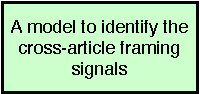
\includegraphics[width=\linewidth]{figures/diagram-RQ.pdf}
    \caption{The relationships between the research questions and the evaluations.}
    \label{fig:diagram}
\end{figure}

% Each one of the vertical columns is described in a different section below.

% This chapters begins with Section~\ref{sec:prop_pipeline} that outlines how we want to take existing works from the framing and similarity research areas.
% Then in Section~\ref{sec:prop_rq1} we target RQ1, giving some insights about some new analysis that we can do that would extend the existing automated framing analysis.
% And then in Section~\ref{sec:prop_rq2} we explain how we can analyse the role of news sources, for the relationship between their alignment and the framing they apply and how the stories are changed over time.



\section{Cross-article framing analysis (RQ1)}
\label{sec:prop_rq1}

% RQ1: framing differences
To address the first Research Question
\textbf{(How can we automatically reveal the framing differences in articles presenting the same event?)}, we aim to resolve two sub-questions separately: the first one analyses the \emph{importance} for the reader of comparing multiple articles to understand the framing that is being applied on the news through the revelation of specific framing signals, and the second one explores \emph{how} we can build a tool to identify these framing signals automatically.
In other words, while the first sub-question deals with the importance for the readers, the second question instead targets the automated detection.
The dependency between the two sub-questions underlines that the second needs the outputs of the first one to know how to label the framing differences.

% we aim to automatically identify \textit{signals of framing} that otherwise would not be noticeable: differences in emphasis and selection of details.
% These signals, while they are defined in the theoretical works, they have not been targeted in the automatic framing analysis.

% Starting with the \textit{emphasis}, we aim to analyse how different articles give importance to specific details.
% While existing works just focus on the usage of loaded terms and repetitions to indicate the presence of emphasis, we can enrich this analysis by seeing how other articles describe the same event.
% Comparing between different articles we can spot differences in the main focus of the article (e.g., the title is an indicator) or look at how the details are presented in a different order to set the priorities for the reader.
% And this can be combined with loaded language analysis, to see how certain details are emphasised and pushed with specific words in very different ways.
% \todo{figure}

% To understand the \textit{selection of details} instead, the idea is to compare the articles and get the common, unique and omitted pieces~\cite{bountouridis2018explaining} and then use some linguistic features (e.g., subjectivity, framing devices) to understand what is their role, may them be full sentences or just specific words that have been added or removed strategically.
% With this analysis, we aim to provide for each article, multiple sides of the same story with an insight into what changes between them.


\subsection{The usefulness of multiple articles (RQ1.1)}
% RQ 1.1: cross-article signals
The first column represents a line of research that is needed to understand how useful is for readers to confront the information available in multiple articles to spot the framing techniques used.
% signals
In order to describe and characterise the framing we started from the literature review to gather concrete manifestations of framing, both in theoretical works and in detection methods.
As we have seen in subsection~\ref{ssec:lit_framing_theory}, different manifestations have been theorised and studied in practical studies.
% what we mean by signal
We name these manifestation \emph{signals} because they are signalling the presence of the framing, which is a abstract concept, but they are tangible and can be seen as concrete features.
For example, loaded language emerges as a signal from specific words that have a strong sentiment, and evokes frames of strength, violence, threat and similar.
Or the strategic omission or inclusion of certain details that have the role of shifting the opinion of the reader.
What we want to investigate is whether we can ease their detection from readers by comparing multiple articles, 
% extend this set of signals by exiting the limitations of a single-article analysis. 
and therefore the specific sub-question is \textbf{What is the contribution of comparing multiple articles to reveal signals of framing?}

% Hypothesis
Our hypothesis is that having multiple articles would allow users to easier detect the framing signals that they are faced with, especially with some of them that are particularly subtle to reveal when just looking at a single article at a time.
% these signals will reveal far more than the single-article framing analysis.
As we described in a position paper~\cite{mensio2020towards}, such signals vary from differences in the emphasis (e.g., different articles focus their headlines on a different detail, or present the story in a different order) to the selection of details (e.g., some articles may decide to omit some parts of the story that is reported by others, or include unnecessary details to push for a certain narrative) or also to different term choices (e.g., being stronger in the language, or evoke specific feelings or related events).
For this reason, we want to test how important it is to see multiple articles that treat the same event to discover their point of view/framing through the signals used in the text.

% % This is is the starting point to identify the differences, with a contrastive analysis. We propose here a set of  that can bring the narrative analysis a step further:
% \begin{itemize}
%     \item The \textbf{main focus} of the compared articles is on a different part or detail of the story: this means that while they are both describing the same broad event, they are trying to emphasise or prioritise two different aspects.
%     % Prioritisation is usually based on negativity / unexpectedness / superlativeness \cite{zahid2019towards}.
%     This signal can be computed by looking at the most similar sentence to the article title (proxy of the emphasis), and seeing how it is represented in other documents.
%     % Two articles that are semantically similar overall (they also have sentence-sentence pairs very similar) focus on different details when the titles are similar to different sentence-level cliques.
    
%     \item \textbf{Ordering}: the compared articles present the same details, but in a different order.
%     Re-ordering events tends to be an efficient way of creating implicit cause-effect relationships. 
%     To do this comparison, it is sufficient to find the crossovers in the sentence-level connections.

%     \item \textbf{Selection of details}:
%     One article is \emph{omitting} certain details that have been reported by other articles, or is describing events that are \emph{corroborated} by other sources, or has \emph{unique parts} that do not occur in other articles~\cite{bountouridis2018explaining}.
%     In addition to seeing which parts are selected or omitted, the narrative analysis can help us to find some insights about them (e.g., the article is omitting subjective statements reported by others, or is describing a background event that others did not include).
%     % For the detection of this case, we rely on the work~\cite{bountouridis2018explaining}.
    
%     \item The articles are \textbf{framing} the narrative in different ways from each other. This manifests through comparing linked sentences to observe the differences in terms of framing features: the considered articles are describing the same events but with different framing and reasoning.
%     One concrete example is the usage of \emph{causality}: one article may contain causality signposting between a pair of sentences that is absent elsewhere.
%     % \item The article uses \textbf{causality as a weapon} (where there is no proof of causality).
%     % An article is expressing causality when there are certain devices (signposting) between two sentences/events.
%     % Different articles may show the causality with different levels, so one sees it as causal and the other one does not link the events.
%     Or as another example, the usage of \emph{specific words} can reveal a specific framing: talking about the same detail or entity, the usage of verbs or adjectives may change.
%     % find strong sentiment and subjective words 
%     % (as adjectives for the same entity, or as verbs).
%     % Detail (e.g. black man instead of just saying man, to add a subtle bias).
%     For detecting such peculiarities, %and comparing them, we can combine the framing signals with 
%     features as Named Entities and subjectivity may be combined.
%     % use features coming from subjective and sentiment analysis.

%     \item The comparison can be also done on the \textbf{subjectivity} of the article: both at the document level (saying that this is an opinion piece, while a similar one is more factual) or at the sentence level, by interweaving this signal with the ones proposed before.
%     % is a \textbf{mix of factual and opinionated / subjective} content: subjectivity values on the full document and on specific sentences.
%     % A sentence is on one article subjective and a similar one on a different article is objective.
%     % Also look at the role of the sentence (commentary, action, background). 

% \end{itemize}

% From the signals in Figure~\ref{fig:comparison}, we can see that the first article pushes the narrative towards \texttt{risk} and other negative frames, to sustain the idea presented in the title ``Britain on Edge''.
% The second article, even though it has a lot of information in common with the first one, is more confident on the preparedness of the National Health Service to face the virus (e.g., \texttt{confidence}, \texttt{expertise}).
% The extraction of these cross-article signals is the first step to finding possible cases of manipulation.

% The expansion and refinement of these signals will help us answer RQ1.1.


% analysis
In order to validate our hypothesis, we will run a \textbf{user study} where participants will be shown different articles that present the same event with some differences.
To test the hypothesis of framing being easier to spot when multiple articles are available, we plan to first present to the user just one article and ask to find the framing signals. Then we show also the second article on the side with different details and ask again.
In both the steps, the input asked from the user is to highlight parts of the article(s) and to say why it is providing a certain view angle, as a free text. To obtain these annotation, users will first be shown with the framing techniques identified in the literature, to understand what they are looking for.
We will then compare the number and type of annotations coming from the two different situations (one singe article or multiple articles).
It is important to divide the annotators of a certain pair of articles in two sub-groups in order to divide the effect of ``seeing again the same article twice'' (unwanted) from ``seeing the article compared to another one'' (wanted). For this reason, if we consider A1 and A2, user U1 will first see A1 then A1+A2, while U2 will first see A2 then A1+A2. In this way we can sum CA1(before)+CA2 for U1 and CA1+CA2(before) for U2 where each observation is done at first sight of the corresponding article (see Figure~\ref{fig:user_study}).

% Hypothesis: users will be able to see more signals in the second phase.

\begin{figure}[!htb]
    \centering
    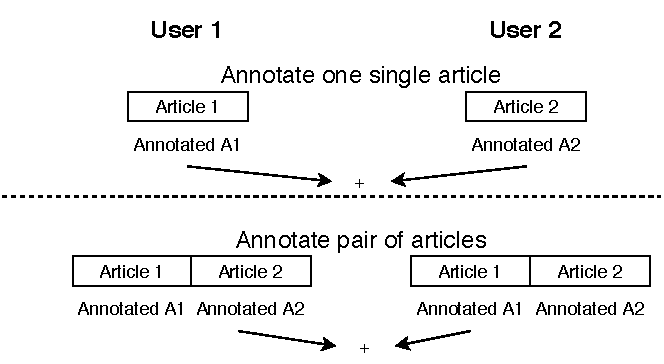
\includegraphics[width=\linewidth]{figures/diagram-user-study-flow.pdf}
    \caption{How to compare the user annotations to exclude effects of second-reading}
    \label{fig:user_study}
\end{figure}
\todo{improve figure to represent better the user study (e.g., annotated pair of articles)}


% requirements
% data (hand-picked samples from sources with different political alignment)
The pairs of articles to be shown will come from a selected subset from clusters of documents that are presenting the same detail, with some differences in the terms used. For this reason they need to be revised and checked.
The clusters will come from articles suggested by AllSides and other news aggregators like Google News, testing both differences from opposite political views as well as articles without any difference in the political bias.
To identify the pairs of documents we plan to use the help from similarity models that, as will be seen in Chapter~\ref{chap:plan}, have been investigated and used to cluster documents and sentences.

% Participants will be presented with two articles and will be asked a set of questions that investigate the effect of having different terms, different details and how user think this is related to try to push for a certain perspective on the events described.

% Do the articles have the same point of view? Do they convey the same message? Title? Details?
% Sentences
% - Do these sentences have different information?
% - Do they provide different perspective?
% - Are there any terms that push for a certain perspective?
% - What is the difference in the intent of communication?
%   - Detail (random, look like professional and detailed, mislead, emphasise on something)
%   - Word choice: emphasise, promote, demote
% if they value the selected differences as signals of the different point of view of the sources (framing), and what they think that the difference is (is it that they are omitting something, commenting, emphasising, other)?

% Or study 2 (better):


% outputs
The annotations will be manually examined with two goals.
First, to see if the annotators (using inter-annotator agreement measures) are able to spot more signals when they have different articles available.
This will prove or disprove our hypothesis that framing can be revealed easier in this setting.
And second, the annotations will be revised manually to bring them back to some categories that represent framing signals. An example could be ``omission of opposing detail'' or ``biased term''. We need to come up with a set of labels that we can assign to the differences pointed out by the users, guided by their descriptions.



\subsection{Automated framing detection (RQ1.2)}
% how would a cross-article framing analysis perform

The second part of the first Research Question requires building and evaluating an automated method to extract the signals identified in the first user study.
Unlike traditional methods of frame detection that mainly rely on extracting features from single articles to build a classification model, we want to use external features that come from the comparison of multiple articles. Such features could be the uniqueness of certain details (sentences or words) when comparing to other articles describing the same event, or including similar words that are used as substitutes in other articles.
The sub-question we address is the following:
\textbf{To what extent can we automatically recognise framing signals using information from multiple documents?}
% Previous research has been focusing on some of the signals, which we can consider as

% implementation
To implement a method that exploits the differences between multiple articles, we need to be able to use the similarities and differences between the considered documents.
For this reason, we plan to rely on the approaches described in the Literature Review~\ref{sec:lit_relationships} where we analysed some methods that are able to find the similarities at different granularities, and expose the differences of the details provided.
% Based on the initial experiments done to see the similarity between documents, we are implementing a processing pipeline that is able to retrieve, process and compare articles.
The step of feature extraction will be based on a pipeline that will process the documents in several steps.
The first step, \emph{retrieval}, keeps collecting articles from multiple sources, and stores them with a unified schema that includes a set of useful fields: headline and body that are needed by linguistic analysis, the source and publication date which are needed for RQ2.
Then the \emph{processing} stage will use NLP libraries with two main objectives: dividing the articles into sentences and compute the embedded semantic representation of both the articles and the sentences.
The articles and sentences embeddings are then used in the last stage, \emph{linking}, which performs clustering at both article and sentence granularity. Furthermore, corroborated and omitted sentences are identified~\cite{bountouridis2018explaining} and this is added to the features.
In this way, articles that cover the same event are brought together and are ready to be compared in their overlap and in their differences.

% how to build on top of the cross-article representation
We need to develop a model that takes features both from the current article and from the linked pieces coming from other articles and performs a classification task to \textit{i)} estimate if the current word is part of a framing signal and \textit{ii)} recognise which specific signal it is part of, inspired by similar approaches that work on single article features~\cite{da2019fine}.
The difference of our approach will be that we plan to use the linked sentences as additional features, to allow the model to learn and exploit the differences between the different article.
Such extension could be obtained by simply adding as features spans of texts that satisfy certain properties (e.g., linked by a certain degree of similarity) or by using \emph{siamese architectures}~\cite{bromley1994signature} that have shown wide application in comparison scenarios.
% https://www.inovex.de/blog/transfer-learning-siamese-networks/
The model will provides as outputs span annotations of framing that will say which framing technique have been used.

\begin{figure}[!htb]
    \centering
    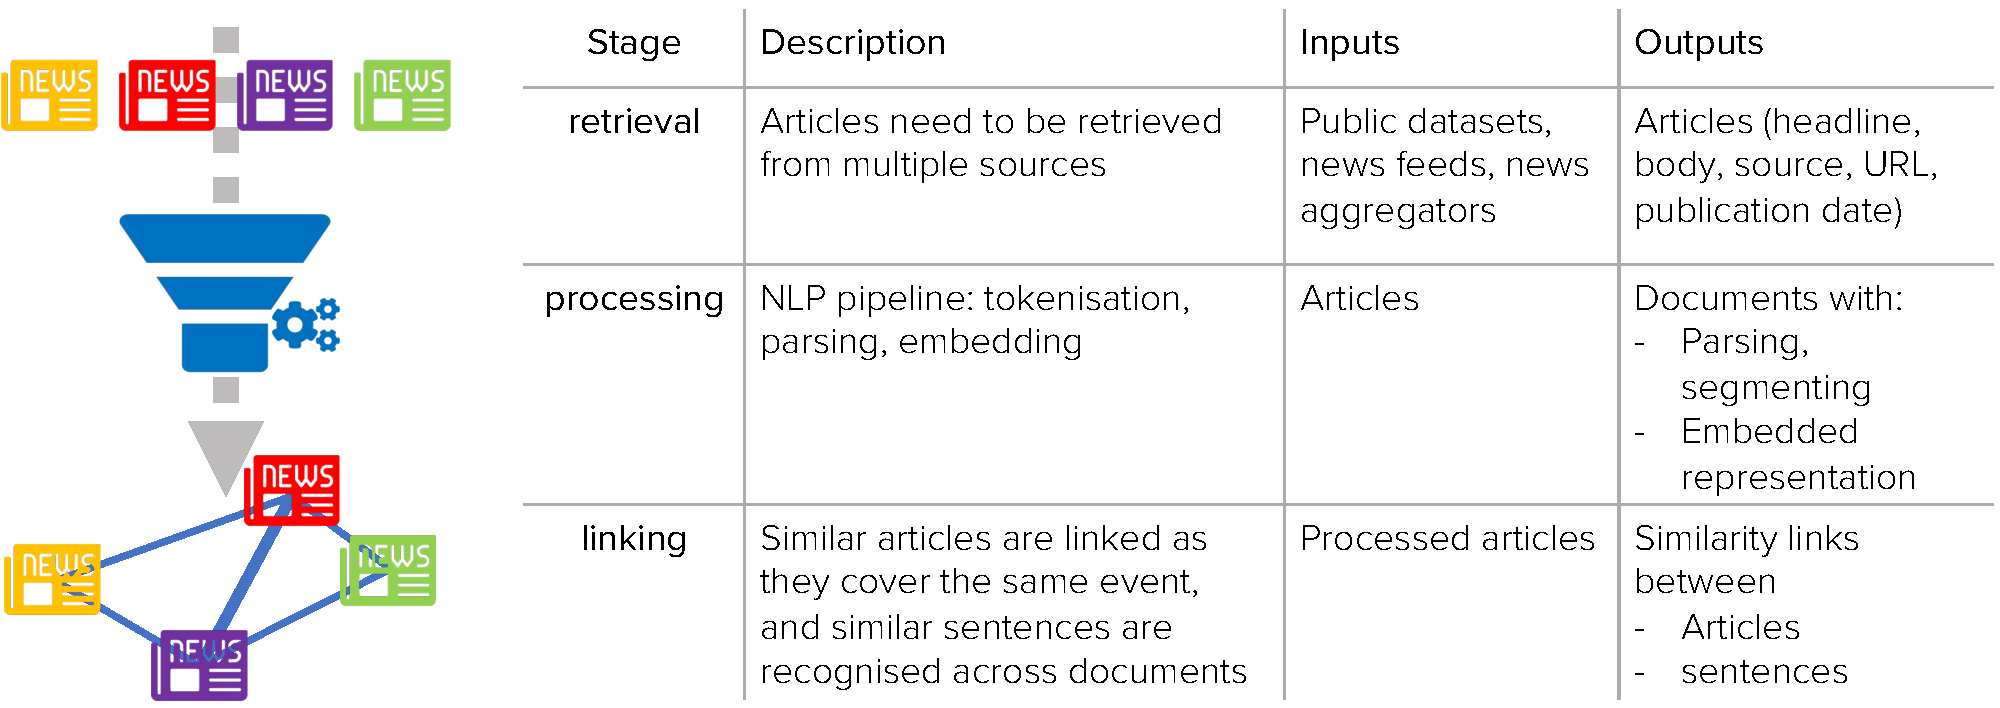
\includegraphics[width=\textwidth]{figures/figure_pipeline.pdf}
    \caption{The processing pipeline that retrieves, processes and links together different articles.}
    \label{fig:pipeline}
\end{figure}

% hypothesis
Our hypothesis is that having the availability of multiple articles would help an automated framing detection model to find more signals of framing.
As the first sub-question analyses the importance for human readers, this analysis wants to see if it is important for the automated detection.
We also hypothesise that some types of framing signals are only detectable by using the external knowledge coming from other articles, which is not used by the existing methods.

% evaluation
To validate or refute our hypothesis, the model will be evaluated by looking at how accurately the spans containing framing differences are identified.
As a comparison, we plan to use models that instead just focus on one single article at a time to extract the features.
For example the complete model will be compared with another version (single-article) that discards the features coming from the comparison.
Or also other models found in the literature that focus on specific types of framing signals (e.g., emphasis detection, loaded terms) will be tested to see if our model (complete or incomplete) is comparable and overtakes them.
% \todo{how to compare to single-article framing datasets? https://ecommons.cornell.edu/handle/1813/39216 from baumer2015testing}
% For some of the framing signals that focus on single articles, there are baselines that are usually only available on specific topics.

% We cannot compare with mostly of them because of the different topics and because the problem

% dataset building
In order to evaluate the model proposed, we will need to collect a larger \textbf{dataset}, where manual annotators will be given the task description and will annotate on document pairs the framing differences according to the schema identified with the first user study.
% (help of pipeline to provide similar articles and candidate words/sentences based on uniqueness)
The pairs of documents will be extracted with the help of the pipeline which will provide articles that are very similar in the content but at the same time have enough differences to be annotated. % (criticality of the threshold)
The annotations will contain the type of signal and also the role/orientation of the two documents (e.g. in an omission signal, one article is \textit{including} and the other is \textit{excluding}, or instead in a term strength variation, one article is \textit{stronger} and the other is \textit{weaker}).
The annotations can be then used both in the multi-article scenario and in the single-article scenario, because different spans will be annotated on the pairs of documents.
For example, if we have an annotation that is highlighting a term that is used with a difference strength, the fact that one term is stronger is available even without having the information of the other article.
This dataset will be made available as a resource paper in order to promote the research on this task.

% outputs
Once this method has been analysed and validated, the detection model will be made available as a tool which help users to see the framing differences between multiple articles.
We plan to put it in an online setting where people will continue to provide training data by correcting or validating the outputs of the tool on new article that have not yet been analysed.
This tool will also be the founding block for the next research questions.

% \subsubsection{Processing Pipeline}\todo{squeeze at the beginning of 4.1.2}
% \label{sec:prop_pipeline}
% The first objective is to build a representation that describes how the articles, and parts of them, are related between each other, together with the framing features coming from the single-article analysis.




% As we can see in Figure~\ref{fig:pipeline}, the processing pipeline is made of different stages:
% % The processing pipeline we propose for this purpose is made of multiple steps:
% \begin{itemize}
%     \item \textbf{preprocessing}: documents are retrieved, cleaned up and fragmented into paragraphs and sentences;
%     \item \textbf{narrative features} are attached to each document, paragraph and sentence belonging to three main types:
%     \emph{structural role} using and highlighting the linguistic devices provided by~\cite{zahid2019towards};
%     \emph{framing features} are extracted (framing and reasoning devices) finding some linguistic representatives from~\cite{gamson1989media,fillmore2006frame};
%     \emph{subjectivity} is computed, and strong word choices are highlighted~\cite{liu2010sentiment};\todo{expand on single-article framing signals}
%     \item \textbf{linking}: \emph{similar articles} are found by using document-level similarity measures: in this way it would be possible to find groups of documents that describe the same events; \emph{similar sentences and paragraphs} are found by sentence-level similarity measures, inside each group of documents: corroborated and omitted sentences are identified~\cite{bountouridis2018explaining}.
% \end{itemize}
% We start with an example of analysis together with the processing pipeline, % that enables this and 
% then we introduce some cross-article signals that highlight the difference in the narratives used.
% First we describe how we think is more reasonable to process the documents (similarity, cliques, hierarchical topic/stories).
% Then we describe which are the  (baseline)(with list).

% At the end of the pipeline, we will have available a representation for the articles that accounts for how they are similar on the document level and at the sentence level.
% % also single-article framing features
% This representation would allow us to navigate between different articles and see their features. We will exploit this representation for answering the two Research Questions, as shown in the following sections.


\section{The role of news sources (RQ2)}
\label{sec:prop_rq2}
% RQ2: also the sources

The purpose of the second research question is to understand the link between the features of the sources and how they frame the news, changing details and taking information from other sources.
While the first research question focused on how to reveal the framing, here we want to investigate how the sources interact with framing. For this purpose, we have two sub-questions that investigate \emph{i)} the relationships between the features of a source and the framing that it uses, and \emph{ii)} how stories are modified and re-framed over time when sources reuse contents from other articles.

\subsection{Source features vs framing (RQ2.1)}
% RQ2.1: relationship with source information
News sources are different and there is a wide variety of them in the media landscape.
A source can have a certain political alignment, be part of a certain news group, have affiliation to certain movements and ideals, or live in a certain country, and we want to do an analysis of the framing techniques across all these features.
% we capture all together as ``affiliation''
Lots of tools and evaluation methods just rely on the provenance of the news, looking at which source published it. The reputation of the sources is a big theme in the credibility domain.
Here we want to analyse the relationship between the features of a news source and how it applies framing differently from others. The sub-question is:
\textbf{Which features of a news source relate with the framing techniques it uses?}
We want to analyse the relationships between the framing choices done by the authors and the news sources where the articles are published. In other words, we want to understand the relationships between the ideological alignment of the news outlets (political alignment, bias, news media groups) and the effective differences contained in the articles.


% With RQ2.1 we ask how does the framing analysis relate with the information of the single outlets (affiliation, newsgroup, bias, partisanship, ...).

% Hypothesis
The hypothesis that we have is that certain features, such as the political alignment, have bigger effects than others, especially when the news topic is about politics.
We want to understand what is the effect of other features as well, and discover which ones influence mostly the framing of the articles written.

% requirement: data on news outlets
In order to test this hypothesis we need two sets of information: the features for each of the sources and the framing analysis.
In the first group, we can use many features:

\begin{itemize}
    \item \textbf{Political alignment}: different ratings exist describing the political leaning of the sources. AllSides, besides comparing articles from different news sources, also provides the bias rating for more than 600 media outlets\footnote{\url{https://www.allsides.com/media-bias/media-bias-ratings}}. Also Media Bias/Fact Check provides the political leaning for more than 3200 news sources. This is probably one of the most important features when analysing the framing about political issues, as their leaning would show slighter support or distancing from actors.
    \item \textbf{News media group/company}: this feature groups together media sources that are part of the same economical group, and therefore would have similar economical reasons in presenting the news about certain topics \footnote{\url{https://en.wikipedia.org/wiki/Category:Newspaper_companies_by_country}}. %https://en.wikipedia.org/wiki/Media_conglomerate
    \item \textbf{Geographical information}: knowing the country and region of a news outlet can provide an analysis of framing across countries to analyse how the same issue is framed differently depending on the position.
    \item \textbf{Factuality and credibility ratings}: there exist multiple ratings that say how factual is the reporting, or how transparent the organisation is in different aspects (MBFC,\footnote{\url{https://mediabiasfactcheck.com/}} NewsGuard\footnote{\url{https://www.newsguardtech.com/}}). All these ratings can instead drive the analysis in seeing how the reputation of a news outlet makes emerge different usage of framing.
\end{itemize}

Instead, to provide the framing analysis, the model from the first Research Question will provide how much each source uses each of the framing techniques, by doing an aggregation on the source level of the analysis of the articles.

% analysis
The analysis will be done by comparing the two sets of features and extracting the most important correlations.
We can apply correlation analysis techniques that will tell us which features relate mostly with which framing technique. 
% Analysis of Variance (ANOVA) techniques~\cite{TODO}
% And once this information is available, we can aggregate a set of framing features (to be defined!!!) by the source of the articles.
\todo{describe more}

% With these two groups of information, we can study their correlation.

% possible outcomes
This correlation analysis will tell us if there are any characteristics of the news sources that make them heavily use framing techniques.
One example that we may discover is that sources heavily biased tend to perform omissions (as seen in~\citet{bountouridis2018explaining}) or use loaded language.


% significance
The outputs of this analysis will hopefully be able to describe the news sources and how they present information.
This would be a step further in making the readers of news more conscious about who they are reading from and guide them, for example, to sources that report the information more completely.
% It will also cast the light more on ... responsibility of 


\subsection{RQ2.2}
% RQ2.2
% what
The last branch of research instead takes the direction of analysing the evolution over time of an event in how it is presented in the media landscape.
We want to track pieces of information and see how different news sources describe them by using different framing techniques and reuse contents from other sources with different modification types.
Our sub-question is the following: \textbf{To what extent can we identify the evolution of the framing of a certain event?}

% why
We want to analyse this phenomenon to explore how the information gets reused and presented under different shapes.
The framing-differences analysis that we plan before does not look at temporal information and therefore has no way of understanding, when two details are similar, which description came first and which one instead is reusing the content from the other.
Although news articles usually cite their sources, there is not much work that explores how the information is modified when reused.


% hypothesis
Our hypothesis is that we will be able to identify patterns between certain sources that take contents from others and perform specific modifications.
It is very likely that, especially small and secondary news outlets sometimes recycle material from other bigger sources, with citations, but they re-adapt some parts for example by changing some wording.
Or on the other side, major headlines that reuse contents from local news outlets that may give too many details for their reporting needs.

% requirements
% Data requirements: timing information.
In order to do this analysis, we need to have precise timing information about the publishing of the articles involved.
In the metadata of the articles usually it it present the publishing date and sometimes also the precise minute.
% Is it reliable? How to manage intervals and not only instants
Relying on this information (that sometimes could be imperfect because of further edits after the first publication), we have the challenge that many articles may indicate the date only and therefore any precise time-dependency could be undetectable.

% how
From the pipeline that gives us similar articles and characterises which parts have been changed, and with the framing analysis that serves to understand which type of modification has been performed, we will conduct this further analysis by ordering documents inside a cluster by publishing time.
Once the documents are sorted, we can then identify the different details, and analyse where do they appear first and how they evolve with time.
Following these details we extract information flows that will give us an understanding of which sources influence others, creating an influence network.
And furthermore we can add to this directed network labels on the edges that correspond to the types of framing modifications that are done.
The analysis to see whether there exist patterns will be conducted by taking the statistics of the framing modifications article-wise and aggregating them to the source level.
In this way we will count between each pair of sources how many times they reused details from others and which types of framing they used.
% And if we also take the timing information (publication time), we can expand this model to characterise the evolution of information, describing how different news sources reuse contents from others and how the details are selected and changed over time.
% \todo{describe analysis}

% outputs
In this way we will show how for example how a certain source, evolves the narrative starting from other sources, merging new elements on its way, emphasising some details, and dropping others.







% Tool for finding other stories on the same event
% External facts not considered
% Highlight words that are used differently
% Tool to analyse the practices of news outlets
% From where do they get info
% How they change it



\chapter{Timeline}
\label{chap:plan}
% Work Plan

This final chapter of this report describes the timeline, considering both the work that has been done up to the current date and the plan for the next two years of research.
While the previous chapter described the methodology and evaluation that is planned, here we describe when each part of the project is expected to be addressed.

\section{Work to date}
% until now: what has been done
% - initial experiments
% - formalisation and problem definition
% - data

During the first year several activities have been done.
Some have been done as initial explorations in the field of research, understanding what other researchers have done, ``getting the hands dirty'' with data and NLP tools.
And their function within the PhD project has been to lead to the Research Questions that we described earlier.
Some other activities have been done to kick start the future experimentation, for example doing data collection of news articles or by beginning to implement some of the stages of the processing pipeline that will be used.
% , with the goal to find and formulate proper Research Questions and to prepare the execution of the proposal.


\subsection{Paper reproduction~\cite{bountouridis2018explaining}}
% Experiment 1
% what
We started by analysing the paper from~\citet{bountouridis2018explaining} which presents a methodology to analyse how much information overlaps between different similar documents, identifying points of information that are corroborated or omitted.
% why
We wanted to analyse this resource because it seems to be going in the broad direction of our project, analysing different presentations in the news of the same event.

% how
The paper has been analysed and reproduced, to get a deep understanding of how it works. The implementation started with the code publicly provided by the authors,\footnote{\url{https://github.com/dbountouridis/InCredible}} but its incompleteness in some stages of the processing (e.g., the creation of the article-level cliques, and all the specific hyperparameters of the algorithms used) required an integration of the codebase.\footnote{\url{https://github.com/MartinoMensio/InCredible}}

% limitations
With the experiments reproduced, we have been able to inspect the cliques of documents and sentences identified by the model, seeing the following limitations:

\begin{itemize}
    % \item Their demo\footnote{\url{http://fairnews.ewi.tudelft.nl/InCredible/}} just shows one specific article as main and one specific clique (not very interesting)
    \item The \emph{document clustering} sometimes splits similar articles over different clusters, or in some cases has different stories that talk about a different detail within the same cluster (e.g., when a news story re-emerges because further details are discovered).
    This can be a consequence of having TF-IDF as underlying method to represent the documents.
    This method is fast and efficient for coarse topic detection, because it is based on bag of words which works well when specific terms that distinguish certain topics.
    But when we need to have a finer-grained clustering such in this case, the limitation of such method may surface because the terms of two political events with the same entities mentioned result in having similar feature vectors.
    \item The \emph{sentence clustering} method provided just says that two sentences are similar, but does not point to which specific words are responsible for the similarities and differences. This would require a framing analysis that in this paper is not included. Furthermore, sentences in a clique are very similar and no big differences have been observed because the similarity metrics is based again on TF-IDF. This method is not robust enough to the usage of synonyms and other variations on the linguistic surface, while at the same time is unable to distinguish two sentences that use the same words but have different meanings because of the sentence structure, so it makes selecting a threshold value very difficult.
    \item The \emph{clique algorithms} are not the best choice for doing clustering when we have the information of how much similar two items are (a real-value is available for the similarity metric). The approach considers an unweighted version of the similarity graph by using a threshold (weights are just used to select the most appropriate clique during their creation), but instead dealing with the original weighted graph would allow better clustering techniques. %, like agglomerative clustering
\end{itemize}


% In addition to these problems, the model described is based on TF-IDF which is not as robust with changes on the linguistic surface (as we saw in the next experiment).
% Models flourished
% This is the motivation for 5.1.2

% And also, it uses the similarity between TF-IDF just with a threshold, modelling the graph and cliques as unweighted (the weights are just used to select the most appropriate clique during their creation).

% role of this experiment
This experiment helped seeing the limitation of this type of work, that belongs to the \emph{similarity} area of research (Section~\ref{sec:lit_relationships}).
This paper provides a great way to analyse the overlap between articles and extracts pieces that have been omitted or that are corroborated, but does not investigate further in the reason behind the selection of what to include or not.
This opened up for further work to:
\begin{enumerate}
    \item investigate how to better represent the documents to provide meaningful similarity metrics;
    \item investigate the works that analyse framing theories and detection;
    \item experiment with document and sentence clustering to bring up differences;
    \item collect data of more recent articles that would be more relevant and interesting.
\end{enumerate}
% \emph{i)} , \emph{ii)} , \emph{iii)} , and \emph{iv)} g.

Apart from these limitations, we are building our processing pipeline on top of this type of analysis, that links together at different granularity levels news articles (document and sentence).


\subsection{Models for similarity analysis}
% Experiment 2
% what
Moving to the problem of representing documents and sentences in a way that captures more the semantic similarity, we decided to analyse closer the existing works, including word embeddings and language models.
We wanted to see in practice how the usage of different representation models would affect the measurements of similarity, experimenting with a small set of articles. 
% finding and exploring more advanced methods to find the similarity between texts by using language models, we experimented on how to use these methods.
% why?
Having a solid base for computing the distances between articles and sentences is a pillar for comparing different articles. The applications of similarity range from document clustering to identification of omitted pieces of information in a cluster, therefore it is very important to use a proper method that is not fooled by usage of synonyms and other linguistic variations in communicating the same information. To study the differences in the language of framing we first need to be able to tell whether two pieces of text are discussing the same information, and distinguish properly degrees of similarity.

% how?
% Specifically on the sentence level, we experimented to see how different models were able to pick similar sentences, by setting up a small benchmark.
We set up a small benchmark where the goal is to find the most similar pairs of sentences coming from selected pairs of news articles which cover the same event. Each model candidate has to tell which 10 most similar pairs of sentences has found, one from one article and one from the other.
The pairs of articles have been chosen manually, by considering three constraints: \textit{i)} description of the same event, \textit{ii)} from different news outlets, \textit{iii)} published near in time, with a maximum distance of one day.
Each model would extract the most similar 10 pairs, and we then compare the pairs provided and their relative order.

The selected models used in the benchmark are the following:
\begin{itemize}
    \item \textbf{TF-IDF}: with a feature size of 2000, with a preprocessing made of lowercasing and tokenizing, without lemmatisation;
    \item \textbf{GloVe-average}: considering GloVe word embeddings trained on the CommonCrawl dataset, and doing an average of the vectors over the sentence;\footnote{\url{https://spacy.io/models/en\#en_core_web_lg}}
    \item \textbf{BERT}: using the most popular embeddings provided by Google Research~\cite{devlin2018bert} with the base uncased pretrained weights;\footnote{\url{https://spacy.io/models/en-starters\#en_trf_bertbaseuncased_lg}}
    \item \textbf{USE}: using sentence embeddings coming from Universal Sentence Encoder~\cite{cer2018universal} which have been specifically trained for sentence similarity\footnote{\url{https://tfhub.dev/google/universal-sentence-encoder/}}
\end{itemize}

In all the cases, the representations from these models have been compared with the cosine similarity.
For each pair of sentences that was provided by any of the models, we listed by manual analysis which differences were contained, by listing the details that changed, or if different words were used.


\begin{figure}[!htb]
    \centering
    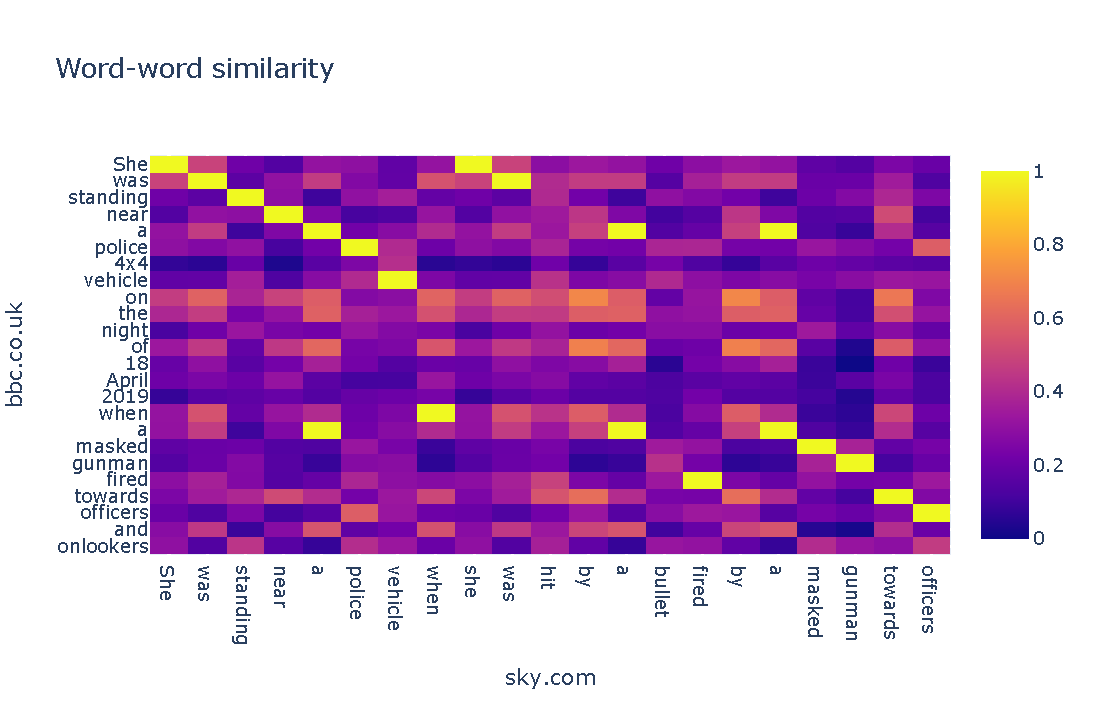
\includegraphics[width=\linewidth]{figures/lyra.pdf}
    \caption{The comparison between two sentences, one from BBC and the other from Sky News, where multiple differences exist.}
    \label{fig:lyra}
\end{figure}
\todo{crop figure, title not needed (already caption)}

An example can be seen in figure~\ref{fig:lyra} that shows a sentence from BBC and one from Sky News, where the differences are the following:

\begin{itemize}
    \item the detail ``4x4'' just appears on the BBC article;
    \item the detail ``on the night of 18 April 2019'' just appears on the BBC article;
    \item Active vs passive sentence ``a masked gunman fired'' vs ``she was hit by a bullet fired by a masked gunman'';
    \item the detail ``a bullet'' just appears in the Sky article;
    \item ``Towards officers and onlookers'' vs ``towards officers'': in the second, the targets of the gunman are just the officers.
\end{itemize}

With this kind of information on the number, type and magnitude of changes contained in different pairs of sentences, we can get a qualitative idea of how the measures of similarity coming from the different models are representative of the effective differences. If a model scores more similar a pair of sentences that appear to us to be less related than another pair, that is a negative sign for that model. 


% Observations
% \todo{rewrite better the observations}
The observations that we have for the TF-IDF model is that
Feature size changes a lot the results.
It requires to be computed on a set of documents all together (which also changes which features are selected), and it is not possible to encode an additional document without changing the representation of the already encoded documents.
We also see that the type of pre-processing affects the results: without a lemmatization step to the pipeline, it is sufficient to change the verb tense to have a different term.
Given these limitations, we find that sentences that are very similar in the meaning but have some differences in the linguistic surface see a drop in their similarity with this model.

Instead considering GloVe-average, we observe in some cases that the measure of similarity provided does not capture substantial changes in the meaning. The problem is that, while it can use wordwise similarity quite well, the sentence structure is not accounted for its representation. The representation is a simple average of the word vectors (e.g. ``Luke insulted John'' results in being equal to ``John insulted Luke'').

For the language models (BERT and USE models), we see a big improvement in the pairs of sentences that come as more similar.
% The values provided are very similar. This per-se is not a problem if some geometric properties are valid (ordering, proportions)
We observe that USE provides values less skewed to the higher end, distributing the similarity values more evenly. The numbers make more sense without any re-scaling technique, and therefore the heatmaps showed in this document come from this model.
It is also the only model considered that is purposely trained on a semantic similarity task, while the other models are able to provide similarity measures just because of how they represent language.


\todo{an example of two pairs where we can see some of the limitations?}

% role of this experiment
This experiment shows the need for a similarity model that accounts for the semantics more than the linguistic surface. And given the continuous progress of language models, we need to be able to switch our choice relatively easily.
For example by looking at the Semantic Textual Similarity benchmark,\footnote{\url{http://nlpprogress.com/english/semantic_textual_similarity.html}} at the moment the best model available is XLNet~\cite{yang2019xlnet} so we will use it for our future experiments.
% this means for us:
% - we need to use a similarity resistant to changes in the linguistic surface
% - we need a measure that is able to represent well the different levels of similarity
% - we must be able to switch the model used easily, in case new public benchmarks for STS show a different winner (example XLNet~\cite{yang2019xlnet}).

The purpose of this experiment is to have a good observation of how different types of models can be effective or not, and to experiment with them to drive the implementation of the processing pipeline.
% Benchmark, availability of code and maybe further measures on our system will decide the final ``winner''.
% Purpose: implementation and building of the pipeline.


\subsection{Sentence clustering and extraction of differences}
% Experiment 3
% what
The next experimentation that we have done regards the usage of the similarity values to group together sentences describing the same details and at the same time study the uniqueness of the words used.
% why
We have seen with the reproduction of the model from \citet{bountouridis2018explaining} that one big limitation of using cliquing techniques over unweighted graphs is that they do not exploit the full power of the distances available, which resulted in having fragmented clusters due to a choice of the ``similar-enough threshold'' that is disputable.
% We have also experimented with different embedding models and we want to use them
% \todo{from here on}
% This comes from the limitation of the first experiment of reproduction of the paper. (from experiment 1)
% (from experiment on similarity)

% how
With this idea, we retrieved some groups of articles that relate to the same event from Google Headlines, which aggregates and clusters together news articles from multiple sources.\footnote{\url{https://www.blog.google/products/news/new-google-news-ai-meets-human-intelligence/}}
These documents are processed with the SpaCy NLP Python library\footnote{\url{https://spacy.io/}} in order to split the documents into sentences and have available different NLP functions (e.g., tokenisation, POS tagging).

% 1. distance computation
Each of the sentences is then passed through a language model which creates a sentence embedding, in this case using the Universal Sentence Encoder because it showed to distribute the similarity values more evenly and is specifically trained for sentence similarity.

% 2. hierarchical clustering (example with diagram)
We then use agglomerative hierarchical clustering for different reasons:
\begin{itemize}
    \item it does not require the specification of the number of clusters wanted, we want to be flexible;
    \item we can truncate the clustering when we reach a certain level of distance between the clusters, or a certain number of clusters;
    \item We can see the evolution of many different features (e.g., number of clusters, size, internal cohesion) while performing the clustering step by step;
    \item we have a graphical representation (dendrogram) which helps inspecting and understanding what is happening;
    \item it has widely been used for similar tasks (e.g., finding related claims~\cite{TODO:meedan_talk_similarity:http://ceur-ws.org/Vol-2607/short4.pdf:or_better})
\end{itemize}

% This clustering algorithm has the following parameters:
% \begin{itemize}
%     \item linkage method: how to choose which clusters to merge. Different strategies exist: Ward: minimise the total within-cluster variance (weighted squared distance between cluster centres). Single: Nearest Point Algorithm. Complete: Farthest Point Algorithm
%     \item distance function: cosine, euclidean, ...
% \end{itemize}
% \todo{describe why ward and cosine look better}

As we can see in Figure~\ref{fig:dendrogram}, we can explore what is the distance required to have different sentences inside the same cluster, and select a certain threshold more consistently.
\begin{figure}[!htb]
    \centering
    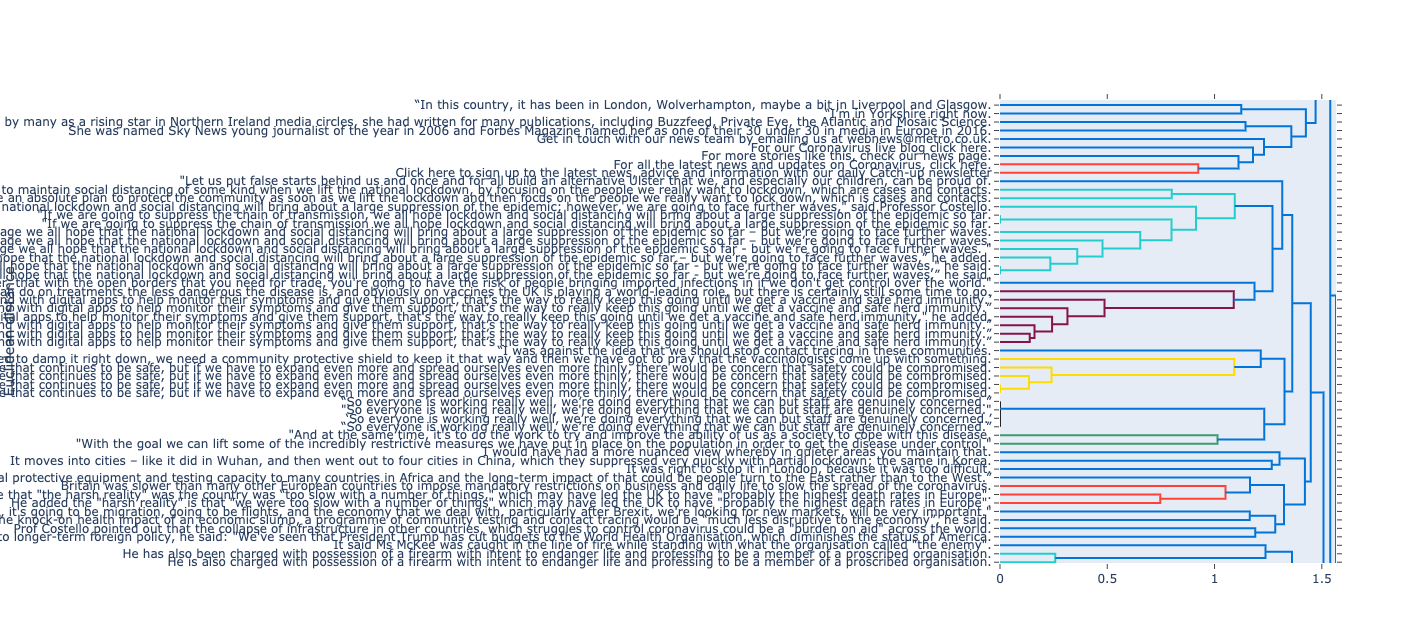
\includegraphics[width=\linewidth]{figures/dendrogram.png}
    \caption{A portion of the dendrogram that shows how different sentences are merged together in the clusters by increasing distance values.}
    \label{fig:dendrogram}
\end{figure}
\todo{redo figure with cosine distance, and higher to be more readable}

Using this type of inspection, we can decide specific threshold values more consistently: we can see what is the required similarity to make two pairs of sentences be in the same cluster.
% \todo{some observations about the distance values and threshold}

% 3. extract degree of uniqueness of words (from pairwise to clusterwise, with bag-of-words or difftool (order matters, duplicates))
% second motivation: highlight the different words and their uniqueness
With this method we create sentence clusters that are very similar in their semantic content, but at the same time have linguistic changes.
With the objective of facilitating an analysis of the differences, we experimented with different methods of highlighting the uniqueness of the words in a cluster.
This can be seen in Figure~\ref{fig:words_uniqueness} where we score each of the words with a scale of uniqueness that is defined as:
$$u_w = 1 - \frac{|\Set{s_i | s_i \in S \land w \in s_i}|}{|S|}$$
where S is the set of sentences considered, $w$ is the word for which to compute the index. The expression compares the sentences of the current cluster where $w$ appears (numerator) with respect to the cluster size.
A value close to $1$ means that the word is used in just a few sentences in the cluster.
This gives a higher value of uniqueness to the word ``deceased'' that just appears in one over three sentences ($u = 2/3$), while ``surgery'' has $u = 0$.

\begin{figure}[!htb]
    \centering
    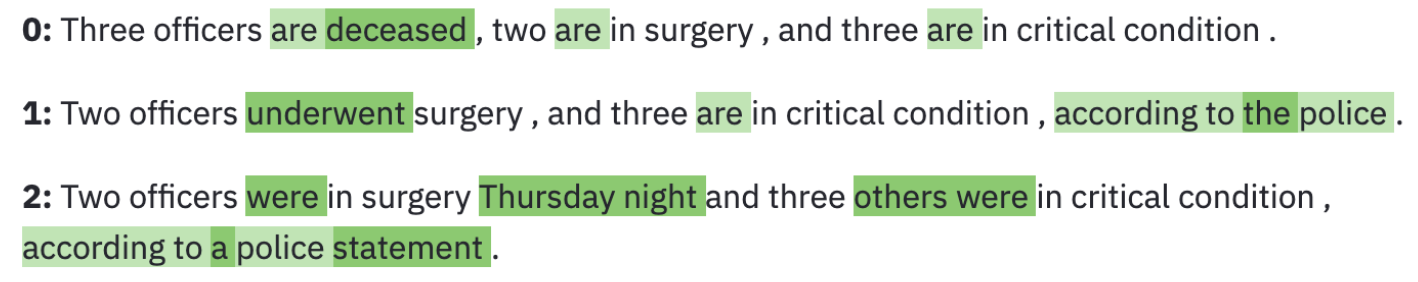
\includegraphics[width=\textwidth]{figures/words_uniqueness.png}
    \caption{A sentence cluster example, where the uniqueness of words in the cluster is highlighted with different shades of green.}
    \label{fig:words_uniqueness}
\end{figure}



% role of this experiment and outcomes
This methodology can be used in our framework to help the preparation of the dataset in different steps.
First of all, during the decision of creating article couples that have to be compared (using at the article-level the same clustering methodology). In this case we will need to use a specific threshold that cuts out unrelated articles but at the same time keeps a considerable number of differences on the document level (not too similar because identical articles, that are a lot, are not useful).
While for the first user study we can exploit hand-curated groups of articles, when doing a larger creation of the dataset we will need to rely on automated techniques.
This methodology could also be used as support for the annotators, in order to see both which sentences are most similar, and the words that differ inside. This would make the annotation process faster and easier.

This experiment needs to be completed, to choose some parameters with better criteria. We want to identify good intervals for the thresholds and parameters (e.g. with euclidean distance around 0.6-1.0 sentences start to have linguistic variations but still very related to the same concepts).

This experiment evidences the need to explore more on the interpretation of the differences, pushing for the user study of RQ1.1.

It serves the RQ1.2 as a first implementation of the processing pipeline by making available different articles and their document and sentence-wise relationships. Building on top of these features, we can then develop the methodology for doing the cross-article framing analysis.




\subsection{Data collection}
% what
We also started collecting, early this year, different type of data that will be useful for the analysis planned.
% why
When looking for data, we are interested by different features.
Firs of all, a wide set of articles is needed, dense in time and from a wide variety of news outlets. We need substantial overlap between articles and the more sources we can include, the better we can observe variation of the framing phenomena.
Another feature that is very important, is to have a good pre-clustered set of articles to help, especially for the first Research Question, the curation of a dataset by knowing that the articles are well related. Then when we will have the document clustering working in action, this feature is not anymore required, but still can serve as benchmark for that stage.
And another desirable feature would be to have articles that come sources with a different opinion, that would be beneficial to create examples especially for the user study, where we want to maximise the occurrence of framing techniques. 

% how
% - google news (more than 500k articles) daily. Some stats about the number of sources involved  TODO: how is it made? What are its properties? Why useful?
Given these requirements and after exploring different news aggregators, we found that Google Headlines Full Coverage feature\footnote{\url{https://www.blog.google/products/news/new-google-news-ai-meets-human-intelligence/}} would fit the requirements of covering a big number of news sources (the \texttt{en-GB} version containing articles from more than 10k domains) and being very dense (an average of 9k new articles each day).
The data comes divided by topics (Latest, United Kingdom, World, Business, Technology, Entertainment, Sports, Science, Health) and inside each topic the articles are grouped in ``stories''. Each story has articles from the most relevant sources (``Top coverage'') and then lists also articles from other less important sources, for an average of 21 articles inside each story.
The stories are created automatically by Google News and this allows it to be always updated and be so diverse in the sources included.
We have captured from mid-march every day the published set of stories, and managed to retrieve more than 700k articles (as of the end of June, and not all the articles listed can be retrieved because of paywalls or other filtering techniques by the publishers).

% - allsides: human-created with interesting framing differences
Another data source that we actively retrieve is AllSides which provides a curated set of ``headlines''\footnote{\url{https://www.allsides.com/story/admin}} where three article with a different political alignment are put together and compared in their difference.
The curators provide a description of how the story gets framed by the considered sources, using natural language.
This description usually contains usage of terms or themes that get mentioned.
At the end of June we have available 4764 headlines, with 13979 articles linked.
Differently from Google Headlines which has different versions for each country, this data is US focused being curated in the US and therefore has a much more limited scope. Also the discussion of bias and framing is mainly focused on political issues, while we want to focus also on other types of differences of opinion.
% role of this specific data
This data, although the description of the differences is not directly parseable, will be used to feed the user study and understand the role of comparing different sides.

% - allnews: standard benchmark, wide adopted (find refs)

% scraping is legal for research: https://aballatore.space/2020/04/01/web-scraping-is-legal/

% role of this
The data collection done in these current months will continue across the PhD, and will be used in different stages of the analysis, serving as the seed to create the labelled dataset that we are aiming to create at the end of the journey of the first Research Question and also providing a wide set of articles from different news sources to empower the studies of the second Research Question.
Having articles from so many different news sources, we can on one side provide some indication of framing for news sources that are not usually targeted by manual framing studies because not enough ``important'', and on the other side be more confident to observe some phenomenon of information flow/re-usage that is the underlying hypothesis for the last sub-question.

\subsection{Formalisation and dissemination}\todo{do we need this?}
% what
The last type of activity carried out during this year has been the presentation of this work to other researchers throughout different events, both internally to the Open University and externally.
% why
The motivation of this activity has been to get some feedback from both people working inside the same research space and also from other fields.
From the first group, we wanted to get an expert opinion and mainly understand if we are missing some related research work that could be helpful.
Instead from the more general-audience group we wanted to understand if this type of research makes sense to them and try to explain more motivationally and in an easier format.

% how
Belonging to the first group, this work has been presented firstly to an internal seminar in KMi on the 25th March, then to the Text2Story workshop part of the ECIR conference as a position paper which was presented in April\footnote{\url{http://text2story20.inesctec.pt/}}.
This position paper~\cite{mensio2020towards} focuses on describing some proposed cross-article signals that would show differences in how stories are narrated.
The proposal described completely in this report has also been presented in the CRC PhD Conference, that is an internal conference for PhD students of KMi and C\&C schools.

Instead belonging to the more wide audience, during June we submitted a poster to the OU PhD Poster Competition which, involving a more general audience, focused more on being simple to understand.

These documents can be found at the end of this file.






\section{Plan}

% realistic
% clearly stated milestones
% dependencies explicit
% contingency planning – risks identified
% timeline – dates
% resources
% skills
% pretty presentation

In Figure~\ref{fig:gantt} we show the time plan, which mirrors the structure of the research questions.

The first phase will target RQ1.1, by doing the user study proposed before. This will require different stages, from the preparation of the data to be annotated and guidelines for the participants, to a small pilot to correct potential errors in the procedure, to the real user study and analysis of the results.

The outputs of the first phase will be needed by the second one, to create and annotate a larger dataset with the specific labels identified in the first study. The implementation of the pipeline is independent from this requirement so it can be done in parallel. The implementation of the detection model will sit on top of the pipeline.

After a month of buffer time, the analysis of the second research question will be faced, with two cycles of data preparation, implementation and analysis.

We plan for each of the groups to use the results of the analysis in papers that will be submitted to upcoming conferences.

The last six months will be dedicated exclusively to writing the thesis.

% \begin{landscape}
\begin{figure}[!htb]
    \centering{
    \resizebox{0.9\textwidth}{!}{
        \begin{ganttchart}[
            % y unit title=1cm,
            % y unit chart=1cm,
            vgrid,
            hgrid,
            time slot format=isodate-yearmonth,
            time slot unit=month,
            % title/.append style={draw=none, fill=barblue},
            % title label font=\sffamily\bfseries\color{white},
            % title label node/.append style={below=-1.6ex},
            % title left shift=.05,
            % title right shift=-.05,
            % title height=1,
            bar/.append style={draw=gray!50, fill=blue!50},
            % bar incomplete/.append style={fill=green}
            % bar height=.6,
            bar label font=\normalsize\color{black!50},
            % group right shift=0,
            % group top shift=.6,
            % group height=.3,
            % group peaks height=.2,
            group/.append style={draw=black, fill=black!50},
            vrule label font=\small,         % <---
            title label font=\small,         % <---
            bar label font=\small, 
            % inline,
  inline bar label node/.append style={
    align=center,
    right=30pt
  },
       ]{2020-07}{2022-09}
       \gantttitlecalendar{year, month}\\
        %   \ganttbar[
        %     progress=100,
        %     bar progress label font=\small\color{barblue},
        %     bar progress label node/.append style={right=4pt},
        %     bar label font=\normalsize\color{barblue},
        %     name=pp
        %   ]{Preliminary Project}{2020-09}{2020-12} \\
        % \ganttset{progress label text={}, link/.style={black, -to}}
        % \ganttgroup{Pipeline}{2020-07}{2020-12} \\
        %     \ganttbar[name=T0]{Implementation}{2020-07}{2020-12} \\
            % \ganttlinkedbar[progress=0]{Task B}{2021-07}{2021-12} \\
        \ganttgroup{RQ1.1}{2020-07}{2020-11} \\
            \ganttbar[]{User study preparation}{2020-07}{2020-09} \\
            \ganttlinkedbar[]{Pilot}{2020-9}{2020-9} \\
            \ganttlinkedbar[]{User Study}{2020-10}{2020-10} \\
            % \ganttbar[progress=0]{RQ1.2: Hypothesis}{2020-07}{2020-12} \\
            \ganttlinkedbar[name=res11]{Results analysis + paper}{2020-10}{2020-11} \\
            % \ganttlink[link mid=.4]{T0}{T12}\\
            % \ganttbar[]{RQ1.2: Analysis}{2021-02}{2021-03} \\
        \ganttgroup{RQ1.2}{2020-07}{2021-05} \\
          \ganttbar[]{Pipeline}{2020-07}{2020-09}\\
            \ganttlinkedbar[name=model12]{Dataset building}{2020-12}{2021-02}\\
            \ganttbar[name=model12]{Model implementation}{2020-12}{2021-02}\\
            % \ganttbar[progress=0]{RQ1.2: Hypothesis}{2020-07}{2020-12} \\
            \ganttlinkedbar[name=output12]{Analysis + paper}{2021-03}{2021-05}\\
            %\ganttlinkedbar[]{Online tool}{2021-03}{2021-04} \\
        
          
        \ganttgroup{RQ2.1}{2021-07}{2021-10} \\
          \ganttbar[name=model21]{Data retrieval and implementation}{2021-07}{2021-08}\\
          \ganttlinkedbar[]{Analysis + paper}{2021-09}{2021-10}\\
          
        \ganttgroup{RQ2.2}{2021-11}{2022-02} \\
          \ganttbar[name=model22]{Implementation}{2021-11}{2021-12}\\
          \ganttlinkedbar[]{Analysis + paper}{2022-01}{2022-02}\\
          
        \ganttgroup{Thesis}{2022-04}{2022-09} \\
          \ganttbar[]{Writing}{2022-04}{2022-09}
          
         \ganttlink[]{res11}{model12}
         \ganttlink[]{output12}{model21}
         \ganttlink[]{output12}{model22}
    \end{ganttchart}}}
    \caption{Gantt chart showing the time plan}
    \label{fig:gantt}
\end{figure}
% \end{landscape}




% \chapter{Conclusion}
\label{chap:conclusion}

asd


% \printbibliography[heading=bibintoc]
% % \bibliography{bibliography}

\bibliographystyle{agsm}
\bibliography{references}

\appendix

\chapter{Appendix Title}

asdasd

\end{document}